\documentclass[12pt, a4paper]{report}

% Include custom styling package strictly conforming to BCSE497J guidelines
\usepackage{vit_template}
\usepackage{natbib}
\bibliographystyle{apalike}

\begin{document}

% -------------------------------------------------------------------------
% PRELIMINARY PAGES (Unnumbered / Roman Numerals)
% -------------------------------------------------------------------------
% 1. Cover Page (Unnumbered)
\begin{titlepage}
\thispagestyle{empty}
\begin{center}
    \vspace*{0.2cm}
    {\fontsize{12}{15}\selectfont\textit{A project report on}}\\[1.2cm]
    
    {\fontsize{20}{25}\selectfont\textbf{A HYBRID TCP/UDP TRANSPORT PROTOCOL FOR FRAGMENTATION-FREE POST-QUANTUM VOICE CHAT}}\\[1.2cm]
    
    {\fontsize{14}{18}\selectfont\textit{Submitted in partial fulfillment for the award of the degree of}}\\[0.8cm]
    
    {\fontsize{22}{27}\selectfont\textbf{Bachelor of Technology in\\COMPUTER SCIENCE AND ENGINEERING}}\\[1.0cm]
    
    {\fontsize{14}{18}\selectfont\textit{by}}\\[0.6cm]
    
    {\fontsize{16}{21}\selectfont\textbf{SREENANDU G (23BCE1120)\\[0.2cm]
    ASHWANTH KUMARAVEL (23BCE1244)\\[0.2cm]
    CAIN MANOJ (23BCE1663)}}\\[1.2cm]
    
    % VIT Logo (rendered cleanly as a vector emblem box if image file is not present)
    \IfFileExists{figures/vit_logo.png}{
        \includegraphics[width=0.45\textwidth]{figures/vit_logo.png}\\[0.6cm]
    }{
        
\begin{tikzpicture}
            \draw[thick, black!80, rounded corners=6pt] (-3.8,-0.9) rectangle (3.8,0.9);
            \node at (0,0.3) {\fontsize{16}{18}\selectfont\textbf{VIT}};
            \node at (0,-0.3) {\fontsize{10}{12}\selectfont\textbf{Vellore Institute of Technology}};
            \node at (0,-0.6) {\fontsize{7}{9}\selectfont(Deemed to be University under section 3 of UGC Act, 1956) \textbf{CHENNAI}};
        \end{tikzpicture}\\[0.8cm]
    }
    
    {\fontsize{16}{20}\selectfont\textbf{SCHOOL OF COMPUTER SCIENCE AND ENGINEERING}}\\[0.8cm]
    
    {\fontsize{12}{15}\selectfont April, 2026}
\end{center}
\end{titlepage}


% 2. Title Page (Unnumbered)
\begin{titlepage}
\thispagestyle{empty}
\begin{center}
    \vspace*{0.8cm}
    {\fontsize{20}{25}\selectfont\textbf{A HYBRID TCP/UDP TRANSPORT PROTOCOL FOR FRAGMENTATION-FREE POST-QUANTUM VOICE CHAT}}\\[1.4cm]
    
    {\fontsize{14}{18}\selectfont\textit{Submitted in partial fulfillment for the award of the degree of}}\\[1.0cm]
    
    {\fontsize{22}{27}\selectfont\textbf{Bachelor of Technology in\\COMPUTER SCIENCE AND ENGINEERING}}\\[1.2cm]
    
    {\fontsize{14}{18}\selectfont\textit{by}}\\[0.8cm]
    
    {\fontsize{16}{21}\selectfont\textbf{SREENANDU G (23BCE1120)\\[0.2cm]
    ASHWANTH KUMARAVEL (23BCE1244)\\[0.2cm]
    CAIN MANOJ (23BCE1663)}}\\[1.4cm]
    
    \IfFileExists{figures/vit_logo.png}{
        \includegraphics[width=0.45\textwidth]{figures/vit_logo.png}\\[0.6cm]
    }{
        
\begin{tikzpicture}
            \draw[thick, black!80, rounded corners=6pt] (-3.8,-0.9) rectangle (3.8,0.9);
            \node at (0,0.3) {\fontsize{16}{18}\selectfont\textbf{VIT}};
            \node at (0,-0.3) {\fontsize{10}{12}\selectfont\textbf{Vellore Institute of Technology}};
            \node at (0,-0.6) {\fontsize{7}{9}\selectfont(Deemed to be University under section 3 of UGC Act, 1956) \textbf{CHENNAI}};
        \end{tikzpicture}\\[0.8cm]
    }
    
    {\fontsize{16}{20}\selectfont\textbf{SCHOOL OF COMPUTER SCIENCE AND ENGINEERING}}\\[0.8cm]
    
    {\fontsize{12}{15}\selectfont April, 2026}
\end{center}
\end{titlepage}


% 3. Declaration by Candidate (Unnumbered)
\thispagestyle{empty}
\begin{center}
    \IfFileExists{figures/vit_logo.png}{
        \includegraphics[width=0.35\textwidth]{figures/vit_logo.png}\\[0.4cm]
    }{
        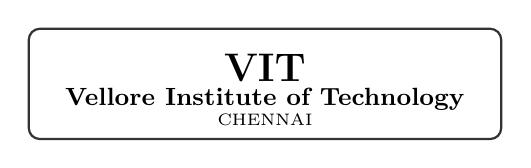
\begin{tikzpicture}
            \draw[thick, black!80, rounded corners=4pt] (-3,-0.7) rectangle (3,0.7);
            \node at (0,0.2) {\fontsize{14}{16}\selectfont\textbf{VIT}};
            \node at (0,-0.2) {\fontsize{9}{11}\selectfont\textbf{Vellore Institute of Technology}};
            \node at (0,-0.45) {\fontsize{6}{8}\selectfont CHENNAI};
        \end{tikzpicture}\\[0.6cm]
    }
    
    \vspace{0.8cm}
    {\fontsize{14}{18}\selectfont\textbf{\underline{DECLARATION}}}\\[1.2cm]
\end{center}

{\fontsize{12}{18}\selectfont\emergencystretch=2em
I hereby declare that the thesis entitled \textbf{“A HYBRID TCP/UDP TRANSPORT PROTOCOL FOR FRAGMENTATION-FREE POST-QUANTUM VOICE CHAT”} submitted by \textbf{SREENANDU G (23BCE1120)}, for the award of the degree of Bachelor of Technology in Computer Science and Engineering, Vellore Institute of Technology, Chennai is a record of bonafide work carried out by me under the supervision of \textbf{Dr. Renuka Devi S.}

I further declare that the work reported in this thesis has not been submitted and will not be submitted, either in part or in full, for the award of any other degree or diploma in this institute or any other institute or university.
}

\vspace{3.5cm}

\noindent
\begin{tabular*}{\textwidth}{@{\extracolsep{\fill}}lr}
    {\fontsize{12}{15}\selectfont Place: Chennai} & \multirow{2}{*}{\textbf{Signature of the Candidate}} \\
    {\fontsize{12}{15}\selectfont Date:} & \\
    & {\fontsize{12}{15}\selectfont\textbf{(SREENANDU G - 23BCE1120)}}
\end{tabular*}


% 4. Certificate by Guide and Examiners (Unnumbered)
\thispagestyle{empty}
\begin{center}
    \IfFileExists{figures/vit_logo.png}{
        \includegraphics[width=0.35\textwidth]{figures/vit_logo.png}\\[0.4cm]
    }{
        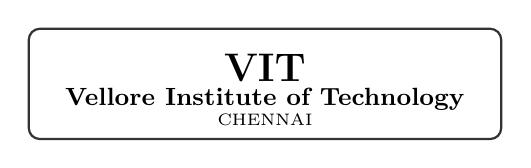
\begin{tikzpicture}
            \draw[thick, black!80, rounded corners=4pt] (-3,-0.7) rectangle (3,0.7);
            \node at (0,0.2) {\fontsize{14}{16}\selectfont\textbf{VIT}};
            \node at (0,-0.2) {\fontsize{9}{11}\selectfont\textbf{Vellore Institute of Technology}};
            \node at (0,-0.45) {\fontsize{6}{8}\selectfont CHENNAI};
        \end{tikzpicture}\\[0.6cm]
    }
    
    \vspace{0.4cm}
    {\fontsize{14}{18}\selectfont\textbf{School of Computer Science and Engineering}}\\[0.6cm]
    {\fontsize{14}{18}\selectfont\textbf{CERTIFICATE}}\\[0.8cm]
\end{center}

{\fontsize{12}{18}\selectfont\emergencystretch=2em
This is to certify that the report entitled \textbf{“A HYBRID TCP/UDP TRANSPORT PROTOCOL FOR FRAGMENTATION-FREE POST-QUANTUM VOICE CHAT”} is prepared and submitted by \textbf{SREENANDU G (23BCE1120)} to Vellore Institute of Technology, Chennai, in partial fulfillment of the requirement for the award of the degree of \textbf{Bachelor of Technology in COMPUTER SCIENCE AND ENGINEERING} is a bonafide record carried out under my guidance. The project fulfills the requirements as per the regulations of this University and in my opinion meets the necessary standards for submission. The contents of this report have not been submitted and will not be submitted either in part or in full, for the award of any other degree or diploma and the same is certified.
}

\vspace{1.5cm}

\noindent
\begin{tabular}{l}
    \textbf{Signature of the Guide:}\\[0.8cm]
    \textbf{Name:} Dr. Renuka Devi S.\\
    \textbf{Date:}
\end{tabular}

\vspace{1.2cm}

\noindent
\begin{tabular*}{\textwidth}{@{\extracolsep{\fill}}lr}
    \textbf{Signature of the Examiner 1} & \textbf{Signature of the Examiner 2}\\[0.8cm]
    \textbf{Name:} & \textbf{Name:}\\
    \textbf{Date:} & \textbf{Date:}
\end{tabular*}

\vspace{1.2cm}

\begin{center}
    {\fontsize{12}{15}\selectfont\textbf{Approved by the Head of Department,}}\\[0.2cm]
    {\fontsize{12}{15}\selectfont\textbf{Department of Computer Science and Engineering}}\\[0.8cm]
    \textbf{Name:}\ \makebox[6cm]{\hrulefill}\\[0.2cm]
    \textbf{Date:}\ \makebox[6cm]{\hrulefill}\\[0.8cm]
    {\fontsize{10}{12}\selectfont\textit{(Seal of School of Computer Science and Engineering)}}
\end{center}


% Frontmatter Page Numbering: Lowercase Roman numerals (i, ii, iii...)
\pagenumbering{roman}
\setcounter{page}{1}

% 5. Abstract (Page i)
\thispagestyle{plain}
\begin{center}
    {\fontsize{14}{18}\selectfont\textbf{\underline{ABSTRACT}}}\\[0.8cm]
\end{center}

{\fontsize{12}{18}\selectfont
Modern encrypted voice-over-IP (VoIP) communications rely heavily on classical key exchange mechanisms such as Diffie-Hellman and elliptic-curve cryptography, which are fundamentally vulnerable to large-scale quantum computers running Shor's algorithm. While post-quantum cryptography (PQC) provides mathematical resilience against ``harvest now, decrypt later'' eavesdropping campaigns, its adoption in real-time interactive voice transport introduces a severe structural networking bottleneck: cryptographic key material is exceptionally large. Standardized lattice-based schemes, such as ML-KEM-768 for key encapsulation and ML-DSA-65 for digital signatures, require a combined handshake payload of 10,842 bytes—more than seven times the typical 1,500-byte Internet Maximum Transmission Unit (MTU). 

When transmitted naively across datagram protocols such as UDP, this payload forces the operating system kernel to slice the handshake into eight separate IPv4 fragments. In lossy wireless environments or networks traversing stateless firewalls and network address translation (NAT) middleboxes, losing even a single fragment invalidates the entire reassembly buffer, causing the overall handshake delivery probability to collapse along a steep $(1-p)^8$ exponential curve. Consequently, at an ordinary packet loss rate of 20\%, naive PQC-over-UDP calls establish successfully only 19 times out of 100 attempts.

To resolve this conflict between cryptographic security and real-time network survivability, this thesis introduces \textbf{HPQV} (Hybrid Post-Quantum Voice), a decoupled dual-channel transport protocol. HPQV routes the oversized, mutually authenticated post-quantum handshake, call signaling, and dynamic key rotation ratchets over a reliable, byte-stream TCP control channel, while streaming low-latency Opus audio frames over an independent UDP data channel. Every voice datagram is encapsulated with an 11-byte authenticated header and encrypted via ChaCha20-Poly1305 AEAD, with per-direction nonce prefix derivation to prevent catastrophic nonce reuse, and is bounded by an explicit 1,200-byte application-level guard with the operating system's Don't-Fragment (DF) socket bit asserted.

We implemented HPQV as a complete userspace prototype in Python 3.11 with low-level C bindings to \texttt{liboqs} and \texttt{libopus}, accompanied by an interactive graphical demonstration interface capable of dynamic in-call loss injection. The protocol was evaluated through extensive empirical packet capture under Linux \texttt{tc netem} kernel impairment, an isolated Opus forward error correction benchmark, and a secondary corroborating discrete-event simulation in NS-3. Empirical packet traces verify that HPQV generates exactly zero IP fragments across all evaluated loss tiers (0\% to 30\%). Under 20\% packet loss, HPQV achieves a 99\% handshake completion rate, maintaining dependable call setup by absorbing packet drop through TCP retransmissions rather than session collapse. Furthermore, Opus in-band FEC improves audio reconstruction quality by 24 dB to 30 dB in segmental SNR compared to packet loss concealment alone. These findings demonstrate that decoupling cryptographic negotiation from datagram voice streaming provides a practical, robust, and standards-aligned pathway for deploying post-quantum security in real-time communications without sacrificing network reliability.
}

\clearpage

% 6. Acknowledgement (Page ii)
\thispagestyle{plain}
\begin{center}
    {\fontsize{14}{18}\selectfont\textbf{ACKNOWLEDGEMENT}}\\[0.8cm]
\end{center}

{\fontsize{12}{18}\selectfont
It is my pleasure to express with a deep sense of gratitude to \textbf{Dr. Renuka Devi S.}, School of Computer Science and Engineering, Vellore Institute of Technology, Chennai, for her constant guidance, continual encouragement, and understanding; more than all, she taught me patience in my endeavor. My association with her is not confined to academics only, but it is a great opportunity on my part to work with an intellectual and expert in the field of Computer Networks and Cryptography.

It is with gratitude that I would like to extend my thanks to the visionary leader \textbf{Dr. G. Viswanathan}, our Honorable Chancellor, \textbf{Mr. Sankar Viswanathan}, \textbf{Dr. Sekar Viswanathan}, and \textbf{Dr. G. V. Selvam}, Vice Presidents, \textbf{Dr. Sandhya Pentareddy}, Executive Director, \textbf{Ms. Kadhambari S. Viswanathan}, Assistant Vice-President, \textbf{Dr. V. S. Kanchana Bhaaskaran}, Vice-Chancellor, \textbf{Dr. T. Thyagarajan}, Pro-Vice Chancellor, VIT Chennai, and \textbf{Dr. P. K. Manoharan}, Additional Registrar, for providing an exceptional working environment and inspiring all of us during the tenure of the course.

Special mention to \textbf{Dr. Viswanathan V}, Dean, \textbf{Dr. Nithyanandam P}, Associate Dean, \textbf{Dr. Suganya G}, Associate Dean, and \textbf{Dr. Sweetlin Hemalatha C}, Associate Dean, School of Computer Science and Engineering, Vellore Institute of Technology, Chennai, for spending their valuable time and efforts in sharing their knowledge and for helping us in every aspect.

In jubilant state, I express ingeniously my whole-hearted thanks to the \textbf{Head of the Department}, B.Tech. Computer Science and Engineering, and the \textbf{Project Coordinators} for their valuable support and encouragement to take up and complete this project report.

My sincere thanks to all the faculty members and staff at Vellore Institute of Technology, Chennai who helped me acquire the requisite technical knowledge. I would like to thank my parents for their unconditional love and support throughout my academic journey. It is indeed a pleasure to thank my teammates—Ashwanth Kumaravel and Cain Manoj—and my friends who encouraged me to take up and complete this task.
}

\vspace{2.5cm}

\noindent
\begin{tabular*}{\textwidth}{@{\extracolsep{\fill}}lr}
    Place: Chennai & \multirow{2}{*}{\textbf{SREENANDU G}} \\
    Date: & \\
    & \textbf{(Reg. No. 23BCE1120)}
\end{tabular*}

\clearpage

% 7. Table of Contents
\phantomsection
\addcontentsline{toc}{chapter}{TABLE OF CONTENTS}
\tableofcontents
\clearpage

% 8. List of Tables
\phantomsection
\addcontentsline{toc}{chapter}{LIST OF TABLES}
\listoftables
\clearpage

% 9. List of Figures
\phantomsection
\addcontentsline{toc}{chapter}{LIST OF FIGURES}
\listoffigures
\clearpage

% 10. List of Acronyms & Abbreviations
\phantomsection
\addcontentsline{toc}{chapter}{LIST OF ACRONYMS}
\thispagestyle{plain}
\begin{center}
    {\fontsize{14}{18}\selectfont\textbf{LIST OF ACRONYMS}}\\[0.8cm]
\end{center}

\noindent
\begin{tabular}{p{3.0cm} p{11.5cm}}
    \textbf{AEAD} & Authenticated Encryption with Associated Data \\
    \textbf{ADR} & Architecture Decision Record \\
    \textbf{CA} & Certificate Authority \\
    \textbf{CBR} & Constant Bit Rate \\
    \textbf{CELT} & Constrained Energy Lapped Transform \\
    \textbf{CI} & Confidence Interval \\
    \textbf{DF} & Don't-Fragment (IPv4 Header Flag) \\
    \textbf{DTLS} & Datagram Transport Layer Security \\
    \textbf{ECMP} & Equal-Cost Multi-Path \\
    \textbf{FEC} & Forward Error Correction \\
    \textbf{FIPS} & Federal Information Processing Standards \\
    \textbf{HKDF} & HMAC-based Key Derivation Function \\
    \textbf{HNDL} & Harvest Now, Decrypt Later \\
    \textbf{HPQV} & Hybrid Post-Quantum Voice \\
    \textbf{IETF} & Internet Engineering Task Force \\
    \textbf{IP} & Internet Protocol \\
    \textbf{KEM} & Key Encapsulation Mechanism \\
    \textbf{LBRR} & Low Bitrate Redundancy \\
    \textbf{LWE} & Learning With Errors \\
    \textbf{MF} & More Fragments (IPv4 Header Flag) \\
    \textbf{MITM} & Man-in-the-Middle \\
    \textbf{ML-DSA} & Module-Lattice-Based Digital Signature Algorithm \\
    \textbf{ML-KEM} & Module-Lattice-Based Key Encapsulation Mechanism \\
    \textbf{MOS} & Mean Opinion Score \\
    \textbf{MTU} & Maximum Transmission Unit \\
    \textbf{NAT} & Network Address Translation \\
    \textbf{NetEm} & Network Emulator (Linux Traffic Control) \\
    \textbf{NIST} & National Institute of Standards and Technology \\
    \textbf{OQS} & Open Quantum Safe \\
    \textbf{PCM} & Pulse-Code Modulation \\
    \textbf{PESQ} & Perceptual Evaluation of Speech Quality \\
    \textbf{PLC} & Packet Loss Concealment \\
    \textbf{PMTU} & Path Maximum Transmission Unit \\
    \textbf{PQC} & Post-Quantum Cryptography \\
    \textbf{QUIC} & Quick UDP Internet Connections \\
    \textbf{RFC} & Request for Comments \\
    \textbf{RND} & Random Number Generator \\
    \textbf{RTP} & Real-time Transport Protocol \\
    \textbf{RTT} & Round-Trip Time \\
    \textbf{SILK} & Skype Speech Audio Codec \\
    \textbf{SIP} & System Integrity Protection / Session Initiation Protocol \\
    \textbf{SNR} & Signal-to-Noise Ratio \\
    \textbf{SRTP} & Secure Real-time Transport Protocol \\
    \textbf{TCP} & Transmission Control Protocol \\
    \textbf{TLS} & Transport Layer Security \\
    \textbf{TTFB} & Time to First Byte \\
    \textbf{UDP} & User Datagram Protocol \\
    \textbf{VoIP} & Voice over Internet Protocol \\
    \textbf{WAP} & Wireless Access Point \\
\end{tabular}

\clearpage

% -------------------------------------------------------------------------
% MAIN THESIS CHAPTERS (Arabic Numerals starting from 1)
% -------------------------------------------------------------------------
\pagenumbering{arabic}
\setcounter{page}{1}

% Chapter 1: Introduction
\chapter{INTRODUCTION}

\section{INTRODUCTION}
Real-time interactive voice communication over packet-switched networks has become the foundational backbone of modern global telecommunications. Over the past three decades, legacy circuit-switched infrastructure (such as the Public Switched Telephone Network, or PSTN) has been largely replaced by Voice-over-IP (VoIP) architectures, WebRTC media pipelines, and decentralized peer-to-peer audio protocols. Unlike non-interactive media streaming or traditional web browsing, real-time voice conversations impose exceptionally stringent physical and perceptual constraints on the underlying transport layer. Human conversation requires interactive latency to remain strictly below 150 milliseconds mouth-to-ear delay, as specified in ITU-T Recommendation G.114. If delay exceeds 200 to 250 milliseconds, conversational flow collapses into disruptive talker overlap and collision.

To achieve this low-latency delivery, voice engines uniformly rely on the User Datagram Protocol (UDP) at the transport layer, commonly paired with the Real-time Transport Protocol (RTP) and secured through the Secure Real-time Transport Protocol (SRTP). UDP avoids the connection establishment delays, retransmission buffering, and head-of-line blocking inherent to the Transmission Control Protocol (TCP). When an audio packet is delayed or dropped due to transient network congestion, retransmitting that packet over TCP is counterproductive: the retransmitted frame arrives dozens or hundreds of milliseconds after its scheduled playback deadline, rendering it useless for audio synthesis while simultaneously stalling the playback buffer for subsequent packets. 

Consequently, real-time voice architectures willingly accept an unreliable, lossy transport substrate. Audio codecs, most notably the standardized Opus codec (RFC 6716), are engineered to conceal lost frames via waveform extrapolation and low-bitrate forward error correction. However, this architectural dependence on UDP introduces a fundamental structural vulnerability when modern voice protocols must be upgraded to withstand the existential threat posed by quantum computation.

\section{THE QUANTUM THREAT AND POST-QUANTUM MIGRATION}
Every established secure voice transport today—including DTLS-SRTP in WebRTC, ZRTP, Signal's voice transport protocol, and TLS-based session control—relies on asymmetric public-key cryptography for endpoint authentication and session key exchange. These protocols depend almost exclusively on two mathematical problems: the integer factorization problem (exemplified by RSA) and the discrete logarithm problem over finite fields or elliptic curves (such as Diffie-Hellman, ECDH with Curve25519, and ECDSA).

In 1994, Peter Shor formulated a quantum algorithm that finds the prime factors of an integer and solves discrete logarithms in polynomial time $\mathcal{O}((\log N)^2 \log \log N \log \log \log N)$ \cite{shor1994algorithms}. On a sufficiently large fault-tolerant quantum computer running error-corrected physical qubits, classical asymmetric cryptography will cease to provide confidentiality or authenticity. While symmetric primitives such as AES-256 and ChaCha20 remain practically secure against quantum cryptanalysis—requiring Grover's algorithm to achieve a quadratic speedup that merely reduces 256-bit security to an effective 128-bit margin—asymmetric key negotiation mechanisms will be completely broken.

This cryptanalytic threat is not a distant prospective issue. Under the ``Harvest Now, Decrypt Later'' (HNDL) operational doctrine, nation-state intelligence agencies and well-resourced adversarial entities are actively intercepting and archiving petabytes of encrypted telecommunication traffic traversing international undersea cables and fiber-optic backbones. Even though adversaries cannot decipher the encrypted voice payloads today, any archived session key exchange negotiated via classical ECDH can be retroactively solved once cryptanalytically relevant quantum computers (CRQCs) become operational. For state secrets, diplomatic communications, proprietary corporate intelligence, and private civic discourse, confidentiality requirements routinely span twenty to thirty years. Encrypted voice sessions recorded today must therefore be secured with quantum-resistant key establishment mechanisms immediately.

In response to this imperative, the National Institute of Standards and Technology (NIST) conducted an intensive eight-year post-quantum cryptography standardization initiative, concluding in 2024 with the formal release of Federal Information Processing Standards (FIPS):
\begin{enumerate}
    \item \textbf{FIPS 203 (ML-KEM):} A module-lattice-based key encapsulation mechanism derived from CRYSTALS-Kyber, serving as the primary standard for quantum-resistant asymmetric key establishment \cite{nist_fips203}.
    \item \textbf{FIPS 204 (ML-DSA):} A module-lattice-based digital signature algorithm derived from CRYSTALS-Dilithium, designed for quantum-resistant digital authentication and integrity verification \cite{nist_fips204}.
\end{enumerate}

While these mathematical constructions withstand both classical and quantum cryptanalysis, their security relies on the hardness of lattice problems (specifically Module Learning With Errors, or M-LWE) over high-dimensional polynomial rings. This algebraic structure imposes a severe physical cost: cryptographic artifacts are orders of magnitude larger than their classical counterparts.

\section{THE CONFLICT: PQC OVERHEAD AND IP FRAGMENTATION}
The crux of this research arises from an irreconcilable conflict between post-quantum payload sizes and the fundamental constraints of datagram networks.

In classical communications, an elliptic-curve Diffie-Hellman key exchange (e.g., X25519) requires exchanging public keys of just 32 bytes, while an Ed25519 signature occupies 64 bytes. The entire classical mutual authentication handshake readily fits into a single, compact UDP packet well under 500 bytes.

In contrast, post-quantum primitives require substantial data transfer. In this work, we deploy the standard NIST security Category 3 parameter sets: ML-KEM-768 for key establishment and ML-DSA-65 for mutual identity authentication. The public parameters and cryptographic outputs exhibit the following dimensions:
\begin{itemize}
    \item \textbf{ML-KEM-768 Public Key:} 1,184 bytes
    \item \textbf{ML-KEM-768 Ciphertext:} 1,088 bytes
    \item \textbf{ML-DSA-65 Public Key:} 1,952 bytes
    \item \textbf{ML-DSA-65 Signature:} 3,309 bytes
\end{itemize}

A fully mutually authenticated handshake requires the calling entity (initiator) to transmit its ephemeral KEM public key, its long-term identity signature public key, and a signature proving ownership. The answering entity (responder) must reply with the encapsulated KEM ciphertext accompanied by a signature over the transcript. Summing these records yields an unprecedented handshake payload:
\begin{align}
    \text{Initiator HELLO} &= 1\ (\text{version}) + 1184 + 1952 + 3309 = 6,445\ \text{bytes} \\
    \text{Responder ACCEPT} &= 1\ (\text{version}) + 1088 + 3309 = 4,397\ \text{bytes} \\
    \text{Total Handshake Payload} &= 6,445 + 4,397 = \mathbf{10,842\ \text{bytes}}
\end{align}

This 10,842-byte security payload must traverse an Internet designed around a standard Ethernet Maximum Transmission Unit (MTU) of 1,500 bytes (and a minimum guaranteed IPv6 MTU of 1,280 bytes). When an application transmits a 6,445-byte or 4,397-byte datagram over standard UDP, the operating system kernel is forced to fragment the datagram at the IP layer.

\begin{figure}[htbp]
    \centering
    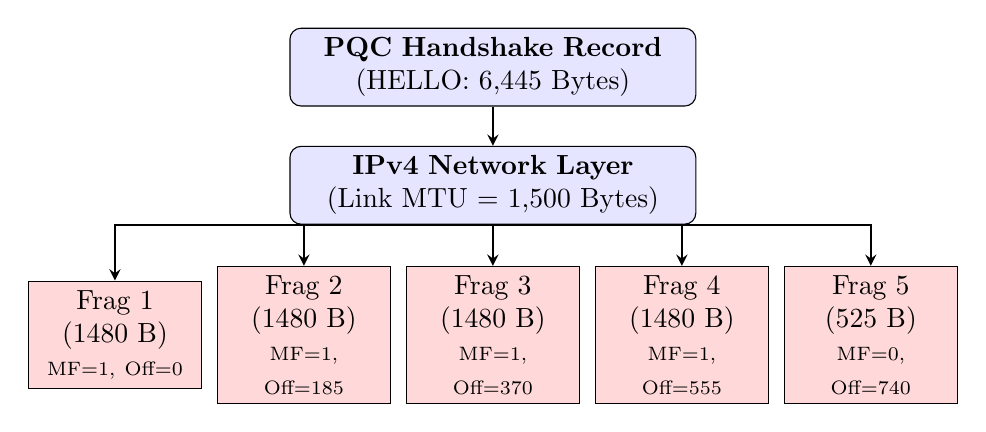
\begin{tikzpicture}[
        every node/.style={align=center},
        mainblock/.style={rectangle, draw, fill=blue!10, text width=14em, align=center, rounded corners, minimum height=2.4em},
        fragblock/.style={rectangle, draw, fill=red!15, text width=5.6em, align=center, minimum height=2.2em},
        conn/.style={thick, ->, >=stealth}
    ]
        \node [mainblock] (app) at (0, 3.0) {\textbf{PQC Handshake Record}\\(HELLO: 6,445 Bytes)};
        \node [mainblock] (ip) at (0, 1.5) {\textbf{IPv4 Network Layer}\\(Link MTU = 1,500 Bytes)};
        
        \node [fragblock] (f1) at (-4.8, -0.4) {Frag 1 (1480 B)\\{\scriptsize MF=1, Off=0}};
        \node [fragblock] (f2) at (-2.4, -0.4) {Frag 2 (1480 B)\\{\scriptsize MF=1, Off=185}};
        \node [fragblock] (f3) at (0, -0.4) {Frag 3 (1480 B)\\{\scriptsize MF=1, Off=370}};
        \node [fragblock] (f4) at (2.4, -0.4) {Frag 4 (1480 B)\\{\scriptsize MF=1, Off=555}};
        \node [fragblock] (f5) at (4.8, -0.4) {Frag 5 (525 B)\\{\scriptsize MF=0, Off=740}};

        \draw [conn] (app) -- (ip);
        \draw [conn] (ip.south) -| (f1.north);
        \draw [conn] (ip.south) -| (f2.north);
        \draw [conn] (ip.south) -- (f3.north);
        \draw [conn] (ip.south) -| (f4.north);
        \draw [conn] (ip.south) -| (f5.north);
    \end{tikzpicture}
    \caption{IPv4 Fragmentation of an Oversized PQC Handshake Datagram across an MTU of 1500 Bytes.}
    \label{fig:ip_frag_overview}
\end{figure}

As illustrated in Figure \ref{fig:ip_frag_overview}, transmitting the initiator's \texttt{HELLO} message results in five IP fragments, while the responder's \texttt{ACCEPT} produces three fragments, yielding eight physical packets for a single exchange. In IP fragmentation, reassembly occurs strictly at the receiving operating system's IP reassembly buffer. Crucially:
\begin{enumerate}
    \item \textbf{All-or-Nothing Reassembly:} UDP provides no selective acknowledgment or fragment-level retransmission. If even a single fragment among the eight is lost in transit, the destination kernel discards the remaining seven fragments upon reassembly timeout. The entire 10,842-byte handshake fails.
    \item \textbf{Exponential Failure Scaling:} Assuming independent packet loss probability $p$, the mathematical probability that an 8-fragment handshake successfully arrives intact is governed by:
    \begin{equation}
        P_{\text{survival}} = (1 - p)^8
    \end{equation}
    At a modest wireless packet loss of $p = 0.20$ (20\%), the survival rate collapses to:
    \begin{equation}
        P_{\text{survival}} = (1 - 0.20)^8 = (0.8)^8 \approx 0.1677\ \ (16.8\%)
    \end{equation}
    Over 83\% of call connection attempts fail completely.
    \item \textbf{Middlebox Pathologies:} Commercial network middleboxes—including NAT gateways, stateless stateful packet inspection firewalls, and Equal-Cost Multi-Path (ECMP) routers—routinely drop out-of-order IP fragments or non-zero offset packets to prevent reassembly buffer exhaustion attacks (e.g., Teardown and Rose attacks) \cite{shannon1984ipfrag}.
\end{enumerate}

Thus, naively injecting post-quantum cryptographic primitives into conventional UDP voice architectures catastrophically undermines the availability and survivability of the telecommunication service.

\section{PROJECT STATEMENT}
This thesis addresses the fundamental problem of network-layer fragmentation in post-quantum encrypted voice telecommunications. Specifically, this work formulates, implements, and evaluates a hybrid transport architecture that decouples control-plane security establishment from data-plane media streaming. By migrating the 10,842-byte post-quantum cryptographic handshake onto a reliable, stream-oriented TCP control channel while constraining encrypted Opus voice datagrams onto an unfragmented UDP data channel capped strictly at 1,200 bytes with the IP Don't-Fragment bit asserted, the system guarantees zero IP fragmentation while preserving real-time conversational latency.

\section{RESEARCH OBJECTIVES}
The primary technical and academic objectives of this project are:
\begin{enumerate}
    \item \textbf{Protocol Architecture Design:} Formulate a decoupled transport protocol (\textbf{HPQV}) combining reliable TCP control framing with low-latency, unfragmented UDP datagram streaming.
    \item \textbf{Post-Quantum Mutual Authentication:} Construct a secure cryptographic handshake deploying ML-KEM-768 and ML-DSA-65 with complete transcript binding (ADR-0002) and out-of-band identity pinning to prevent man-in-the-middle attacks.
    \item \textbf{Key Derivation and Directional Nonce Isolation:} Implement an HKDF-SHA256 expansion scheme that derives independent 32-byte session keys and distinct 4-byte directional nonce prefixes, eliminating symmetric cipher nonce reuse vulnerabilities in ChaCha20-Poly1305.
    \item \textbf{Enforced Datagram Invariant:} Establish an enforced application-level boundary of 1,200 bytes per voice packet, accompanied by explicit operating system configuration of the IP Don't-Fragment (DF) bit.
    \item \textbf{Audio Resilience Engine:} Integrate the Opus codec with in-band Low Bitrate Redundancy (LBRR) Forward Error Correction and a heap-based jitter buffer to mitigate packet drop and network jitter.
    \item \textbf{Full Userspace Prototype Implementation:} Develop a clean, modular implementation in Python 3.11 with low-level C bindings, complete with an interactive graphical user interface featuring real-time, in-call loss injection.
    \item \textbf{Multi-Tiered Empirical Benchmarking:} Validate the protocol across a reproducible, containerized testbed utilizing Linux Traffic Control (\texttt{tc netem}) for physical kernel measurement (Track 2) and NS-3 discrete-event network modeling (Track 3) against pure TCP and simulated QUIC baselines.
\end{enumerate}

\section{SCOPE AND BOUNDARIES}
To establish realistic boundaries for an academic B.Tech engineering thesis, the scope of this project is defined as follows:
\begin{itemize}
    \item \textbf{Target Topology:} Point-to-point (two-party) interactive voice communication over IPv4 local and wide-area networks. Multi-party conferencing (e.g., Selective Forwarding Units) is left for future expansion.
    \item \textbf{Identity Infrastructure:} Peer identity public keys are pinned out-of-band via trusted configuration files, matching the operational security models of WireGuard and SSH. Integration with an automated Public Key Infrastructure (PKI) or X.509 Certificate Authorities is excluded.
    \item \textbf{Cryptographic Primitives:} Evaluation focuses strictly on standardized lattice-based algorithms (ML-KEM-768 and ML-DSA-65). State-machine signature schemes (e.g., LMS/XMSS) and code-based schemes (e.g., Classic McEliece) are outside the primary prototype scope.
    \item \textbf{Network Environment:} Primary physical evaluations are conducted across virtualized network namespaces and containerized loopback interfaces with MTU pinned to 1,500 bytes to ensure rigorous, reproducible loss and delay control.
\end{itemize}

\section{ORGANIZATION OF THE REPORT}
The remainder of this report is structured as follows:
\begin{itemize}
    \item \textbf{Chapter 2 (Literature Survey):} Reviews theoretical foundations of post-quantum cryptography, real-time transport protocols (RTP, SRTP, WebRTC, QUIC), empirical studies on IP fragmentation middlebox pathologies, and audio quality assessment models.
    \item \textbf{Chapter 3 (System Architecture):} Presents the complete mathematical and architectural specification of the HPQV protocol, including wire framing, mutual authentication handshake mechanics, key ratcheting, and jitter buffer operation.
    \item \textbf{Chapter 4 (Implementation Details):} Details the software engineering architecture, core Python modules, C library bindings, socket-level flags, GUI development, and the 53-case automated verification test suite.
    \item \textbf{Chapter 5 (Experimental Methodology):} Describes the multi-tiered evaluation framework, containerized Docker environment, Linux NetEm configuration, NS-3 simulation calibration, and mathematical formulations for metrics.
    \item \textbf{Chapter 6 (Results and Discussion):} Analyzes empirical findings across fragment counts, handshake survival rates, connection setup latencies, FEC recovery SNR, and NS-3 comparative curves, followed by a critical engineering discussion.
    \item \textbf{Chapter 7 (Conclusion and Future Work):} Summarizes major research findings, validates project deliverables against initial objectives, and outlines future research avenues.
    \item \textbf{Appendices \& References:} Provides exhaustive wire format layouts, mathematical derivations, reproducible environment commands, core code listings, test suite catalogs, and APA references.
\end{itemize}


% Chapter 2: Literature Survey & Background
\chapter{LITERATURE SURVEY AND BACKGROUND}

\section{INTRODUCTION}
The transition to post-quantum secure communications requires reassessing foundational assumptions across network protocol design. While modern cryptographic literature has extensively examined the computational throughput of post-quantum algorithms on server-grade and embedded microprocessors, the network transport layer has received comparatively less scrutiny. In particular, real-time interactive voice applications operate under fundamentally different constraints than bulk data transfers or episodic web browsing. 

This chapter presents a comprehensive literature survey examining four interconnected domains: the theoretical foundations of lattice-based post-quantum cryptography; the state-of-the-art in post-quantum transport layer protocols; the architectural mechanics of real-time voice transport; and the network-layer pathologies associated with IP fragmentation and middlebox interference. The chapter concludes with a systematic gap analysis delineating why existing solutions fail to provide reliable, fragmentation-free post-quantum voice transport.

\section{THEORETICAL FOUNDATIONS OF POST-QUANTUM CRYPTOGRAPHY}

\subsection{Quantum Computing and the Vulnerability of Classical Cryptography}
Classical public-key cryptography rests upon the presumed computational intractability of number-theoretic problems. The RSA cryptosystem relies on the factoring of large composite integers $N = p \cdot q$. The Diffie-Hellman key exchange, ElGamal encryption, and Elliptic Curve Cryptography (ECC) depend on the discrete logarithm problem: given a cyclic group $G$, a generator $g \in G$, and an element $y = g^x$, determine the integer exponent $x$.

In 1994, Peter Shor established that both the integer factorization problem and the discrete logarithm problem belong to the complexity class $\text{BQP}$ (Bounded-error Quantum Polynomial time) \cite{shor1994algorithms}. Shor's algorithm formulates discrete logarithms and integer factorization as instances of the hidden subgroup problem over abelian groups. By utilizing the Quantum Fourier Transform (QFT), a quantum computer evaluates the periodicity of the modular exponentiation function $f(a) = g^a \pmod N$ in quantum superposition across $2n$ qubits:
\begin{equation}
    |\psi\rangle = \frac{1}{\sqrt{2^m}} \sum_{a=0}^{2^m - 1} |a\rangle |g^a \pmod N\rangle
\end{equation}
Applying the inverse Quantum Fourier Transform to the state register yields constructive interference at rational approximations of the period $r = \text{ord}(g)$, allowing classical continued fractions to extract $r$ in polynomial time $\mathcal{O}((\log N)^2 \log \log N)$. 

Because elliptic curve scalar multiplication is an abelian group operation, Shor's algorithm solves elliptic curve discrete logarithms in $\mathcal{O}(n^3)$ operations using only $\mathcal{O}(n)$ logical qubits. Consequently, standardized curves such as NIST P-256 and Curve25519 offer precisely zero asymptotic security against a cryptanalytically relevant quantum computer.

\subsection{Lattice-Based Cryptography and Learning With Errors (LWE)}
To secure communications against quantum cryptanalysis, cryptographers have turned to alternate mathematical structures. Among all evaluated post-quantum families—including code-based, isogeny-based, hash-based, and multivariate quadratic cryptography—lattice-based cryptography has emerged as the premier foundation due to its balanced efficiency, strong worst-case to average-case hardness reductions, and mathematical maturity.

A lattice $\Lambda \subset \mathbb{R}^m$ is a discrete additive subgroup defined by the set of all integer linear combinations of $n$ linearly independent basis vectors $\mathbf{b}_1, \dots, \mathbf{b}_n \in \mathbb{R}^m$:
\begin{equation}
    \Lambda(\mathbf{B}) = \left\{ \sum_{i=1}^n x_i \mathbf{b}_i \;\middle|\; x_i \in \mathbb{Z} \right\}
\end{equation}
The security of lattice primitives reduces to the conjectured worst-case hardness of geometric lattice problems, such as the Shortest Vector Problem ($\text{SVP}_\gamma$) and the Closest Vector Problem ($\text{CVP}_\gamma$), for which no known classical or quantum algorithm achieves polynomial time for polynomial approximation factors $\gamma$.

In 2005, Oded Regev introduced the Learning With Errors (LWE) problem \cite{shor1994algorithms}. For a prime modulus $q$, dimension $n$, and an error distribution $\chi$ over $\mathbb{Z}_q$, the search LWE problem asks an adversary to reconstruct a secret vector $\mathbf{s} \in \mathbb{Z}_q^n$ given a collection of noisy inner products:
\begin{equation}
    (\mathbf{a}_i, b_i = \langle \mathbf{a}_i, \mathbf{s} \rangle + e_i) \in \mathbb{Z}_q^n \times \mathbb{Z}_q
\end{equation}
where $\mathbf{a}_i \leftarrow \mathcal{U}(\mathbb{Z}_q^n)$ and $e_i \leftarrow \chi$. While standard LWE offers robust security, it incurs quadratic space overhead $\mathcal{O}(n^2)$ because matrix $\mathbf{A} \in \mathbb{Z}_q^{m \times n}$ must be transmitted explicitly.

To overcome this bandwidth overhead, Ring-LWE and Module-LWE (M-LWE) define operations over polynomial quotient rings $R_q = \mathbb{Z}_q[X] / (X^n + 1)$, where $n$ is a power of two. In Module-LWE, secrets and errors are vectors of polynomials over $R_q^k$, striking an optimal trade-off between algebraic structure, security assurances, and compact representation.

\subsection{NIST Post-Quantum Cryptography Standards}
Following a multi-year global evaluation, NIST finalized the first standardized post-quantum algorithms in August 2024:

\subsubsection{FIPS 203: Module-Lattice Key Encapsulation Mechanism (ML-KEM)}
Derived from the CRYSTALS-Kyber submission, ML-KEM is parameterized by ring degree $n=256$, modulus $q=3329$, and module rank $k \in \{2, 3, 4\}$ \cite{nist_fips203}. For NIST Security Category 3 (equivalent to AES-192 security), ML-KEM-768 utilizes $k=3$ and error parameter $\eta_1 = \eta_2 = 2$.
\begin{itemize}
    \item \textbf{Key Generation:} Generates seed $d \in \{0,1\}^{256}$, derives matrix $\hat{\mathbf{A}} \in R_q^{k \times k}$ via SHAKE-128, samples secret error vectors $\mathbf{s}, \mathbf{e} \leftarrow \beta_\eta^k$, and computes public key $\mathbf{t} = \hat{\mathbf{A}}\mathbf{s} + \mathbf{e}$. The serialized public key occupies $12 \cdot k \cdot n / 8 + 32 = 1,184$ bytes.
    \item \textbf{Encapsulation:} Given public key $\mathbf{t}$, the sender samples random message $m \in \{0,1\}^{256}$, samples randomness $\mathbf{r}, \mathbf{e}_1, e_2$, and computes ciphertext $\mathbf{u} = \hat{\mathbf{A}}^T \mathbf{r} + \mathbf{e}_1$ and $v = \mathbf{t}^T \mathbf{r} + e_2 + \lceil q/2 \rfloor m$. Ciphertext compression produces an output size of $10 \cdot k \cdot n / 8 + 4 \cdot n / 8 = 1,088$ bytes.
    \item \textbf{Decapsulation:} Reconstructs shared key $K$ via the Fujisaki-Okamoto transform, providing IND-CCA2 security against active chosen-ciphertext attacks.
\end{itemize}

\subsubsection{FIPS 204: Module-Lattice Digital Signature Algorithm (ML-DSA)}
Derived from CRYSTALS-Dilithium, ML-DSA is based on the Fiat-Shamir with Aborts framework over module lattices \cite{nist_fips204}. For Category 3 security, ML-DSA-65 employs matrix dimensions $(k, \ell) = (6, 5)$, modulus $q = 8380417$, and polynomial degree $n=256$.
\begin{itemize}
    \item \textbf{Signing Mechanism:} Computes commitments $\mathbf{w} = \mathbf{A}\mathbf{y}$, extracts high bits $\mathbf{w}_1$, hashes the message and $\mathbf{w}_1$ to derive challenge $c$, and computes response $\mathbf{z} = \mathbf{y} + c\mathbf{s}_1$. Rejection sampling ensures that the distribution of $(\mathbf{z}, c)$ is strictly independent of the secret key $(\mathbf{s}_1, \mathbf{s}_2)$.
    \item \textbf{Key and Signature Sizes:} The serialized public key $\mathbf{t}_1$ requires 1,952 bytes, while the digital signature $(\tilde{c}, \mathbf{z}, \mathbf{h})$ occupies 3,309 bytes.
\end{itemize}

\section{STATE-OF-THE-ART IN TRANSPORT LAYER PQC PROTOCOLS}

\subsection{Post-Quantum TLS 1.3}
Transport Layer Security (TLS 1.3, RFC 8446) is the dominant security protocol for Internet data transfer \cite{rfc8446}. Research into post-quantum TLS has primarily focused on benchmarking hybrid and pure PQC key exchange. 

Sosnowski et al. (2023) evaluated post-quantum TLS 1.3 handshakes across diverse network conditions \cite{sosnowski2023performance}. Their findings revealed that while ML-KEM-768 key encapsulation imposes minimal CPU overhead on modern x86\_64 processors ($\approx 0.1\text{ ms}$), the transmission of large PQC public keys in the \texttt{ClientHello} message frequently triggers TCP segmentation. On low-bandwidth or lossy connections, segment drops during connection establishment induce TCP retransmission timeouts, significantly increasing the Time to First Byte (TTFB).

Crockett, Paquin, and Stebila (2019) prototyped post-quantum and hybrid algorithms within OpenSSL and BoringSSL \cite{crockett2019prototyping}. Their analysis demonstrated that post-quantum digital signatures (such as Dilithium and Falcon) introduce severe network penalties during the TLS certificate exchange: because standard X.509 certificate chains contain multiple signatures, transmitting a PQC certificate chain expands the handshake by 7 to 15 kilobytes, forcing the initial TCP congestion window ($\text{initcwnd} = 10$) into early congestion and multi-round-trip serialization delays.

\subsection{Post-Quantum QUIC}
QUIC (RFC 9000) is a UDP-based, stream-multiplexed transport protocol integrated with TLS 1.3 encryption (RFC 9001) \cite{rfc9000, rfc9001}. Because QUIC operates over UDP, it eliminates TCP head-of-line blocking across independent application streams. 

Kempf et al. (2024) conducted an exhaustive empirical investigation titled ``A Quantum of QUIC: Dissecting Cryptography with Post-Quantum Insights'' \cite{kempf2024quantum}. They analyzed the behavior of QUIC implementations when executing post-quantum handshakes. A critical limitation emerged: standard QUIC enforces an anti-amplification limit (RFC 9000, Section 8.1). Before an endpoint's IP address is validated, a QUIC server must not transmit more than three times the volume of data received from the client ($3\times$ amplification limit). When large post-quantum public keys or certificates are transmitted, the server's handshake response frequently exceeds this threshold, forcing the server to pause transmission and wait for an extra round-trip validation from the client.

Dong and Wang (2025) proposed EPQUIC, optimizing post-quantum QUIC handshakes by caching public keys and parallelizing polynomial arithmetic \cite{dong2025epquic}. However, EPQUIC focuses on client-server web workloads; it does not address real-time bidirectional audio streaming where connection establishment must immediately yield an uninhibited, low-jitter datagram channel.

\subsection{TurboTLS and Transport Workarounds}
In 2024, Aguilar-Melchor et al. introduced TurboTLS \cite{aguilar2024turbotls}. TurboTLS recognized that large post-quantum handshakes exacerbate latency. To accelerate connection establishment, TurboTLS initiates communication over UDP and TCP simultaneously: an opportunistic UDP handshake packet is transmitted alongside a parallel TCP SYN. If the UDP packet arrives without packet loss, the handshake completes in a single round trip; if packet loss or middlebox filtering occurs, the connection falls back transparently to the parallel TCP stream.

While TurboTLS shares our concept of combining TCP and UDP, its architectural objective is fundamentally different from this thesis:
\begin{itemize}
    \item \textbf{TurboTLS Objective:} Optimizing connection establishment \textit{latency} for web requests by speculatively racing UDP against TCP. Once established, application data flows exclusively over TLS/TCP.
    \item \textbf{HPQV Objective:} Preventing \textit{network-layer fragmentation} of oversized post-quantum handshakes while permanently preserving UDP datagram transport for real-time voice frames. In HPQV, TCP and UDP do not race; they execute distinct functional roles in parallel throughout the lifetime of the call.
\end{itemize}

\section{REAL-TIME VOICE TRANSPORT PROTOCOLS}

\subsection{RTP, SRTP, and WebRTC Architectures}
Real-Time Transport Protocol (RTP, RFC 3550) provides end-to-end network transport functions for streaming audio and video \cite{rfc3550}. RTP packets carry an unencrypted 12-byte header containing synchronization source (SSRC) identifiers, monotonic sequence numbers, and media timestamps to allow receivers to reconstruct playout timing and detect packet loss.

Secure RTP (SRTP, RFC 3711) encrypts the RTP payload and authenticates the entire packet using symmetric cryptography \cite{rfc3711}. In standard WebRTC implementations, SRTP session keys are negotiated dynamically over UDP via Datagram Transport Layer Security (DTLS-SRTP, RFC 5764). 

The reliance on DTLS over UDP creates a fatal failure mode when post-quantum primitives are introduced. DTLS implements its own user-space fragmentation and retransmission timer layer to transmit records exceeding the MTU. However, when an oversized DTLS record (e.g., 6,445 bytes of ML-KEM/ML-DSA material) is split across multiple UDP packets, each packet is subject to independent drop probabilities. Because DTLS uses coarse retransmission timers (typically initialized to 1.0 second), a dropped handshake fragment stalls call setup by seconds—causing users to hang up before the call establishes.

\section{IP FRAGMENTATION MECHANISMS AND MIDDLEBOX PATHOLOGY}

\subsection{Mechanics of IPv4 Fragmentation}
The Internet Protocol was designed to interconnect heterogeneous networks with divergent Maximum Transmission Units (RFC 791). In IPv4, when a packet's length exceeds the MTU of an egress interface, the router or host kernel fragments the payload into multiple smaller IP datagrams, as governed by three header fields:
\begin{enumerate}
    \item \textbf{Identification (16 bits):} A unique integer assigned by the sender to correlate all fragments belonging to a single original datagram.
    \item \textbf{Flags (3 bits):} Includes the Don't-Fragment (DF) bit (bit 1) and the More-Fragments (MF) bit (bit 2). If DF is asserted ($\text{DF}=1$) and packet length exceeds the MTU, the packet is discarded and an ICMP Fragmentation Needed message is returned. If $\text{DF}=0$, the packet is segmented, setting $\text{MF}=1$ for all fragments except the final fragment ($\text{MF}=0$).
    \item \textbf{Fragment Offset (13 bits):} Measures the byte offset of the fragment payload relative to the original unfragmented datagram, expressed in units of 8-byte blocks.
\end{enumerate}

\subsection{Middlebox Vulnerabilities and Empirical Failure Modes}
Extensive empirical networking studies confirm that IP fragmentation is highly fragile in modern production networks. In their landmark empirical analysis ``Beyond Folklore: Observations on Fragmented Traffic,'' Shannon, Moore, and Claffy (2002) measured wide-area traffic and demonstrated that fragmented IP packets suffer drastically higher drop rates than unfragmented packets \cite{shannon1984ipfrag}.

This heightened failure rate stems from several systemic middlebox behaviors:
\begin{enumerate}
    \item \textbf{Stateless Filtering and Firewall Discard:} Transport layer headers (such as UDP source and destination ports) reside exclusively in the first fragment ($\text{Offset}=0$). Subsequent fragments ($\text{Offset} > 0$) contain only raw IP payload without transport headers. Network firewalls executing port-based filtering policies cannot inspect ports in trailing fragments. To prevent blind bypass attacks, firewalls frequently drop all non-zero offset fragments unconditionally.
    \item \textbf{NAT Table Exhaustion:} Network Address Translation (NAT) gateways must rewrite IP headers and transport checksums. When fragments arrive out of order, the NAT device must buffer initial fragments until the offset-zero packet arrives to identify the port mapping. Under heavy traffic or denial-of-service conditions, NAT fragment reassembly tables exhaust their memory limits, discarding pending fragments.
    \item \textbf{ECMP Load Balancing Inconsistencies:} Equal-Cost Multi-Path (ECMP) switches route traffic by hashing the 5-tuple (Source IP, Destination IP, Protocol, Source Port, Destination Port). Because non-zero fragments lack port numbers, ECMP routers hash only the IP addresses, frequently routing different fragments of the same datagram across divergent physical paths with unequal latencies, leading to fragment reassembly buffer timeouts at the receiver.
\end{enumerate}

\section{AUDIO CODING AND RESILIENCE MECHANISMS}

\subsection{The Opus Audio Codec (RFC 6716)}
The standardized Opus codec combines technologies from Skype's SILK codec (specialized for human voice via Linear Predictive Coding) and Xiph.Org's CELT codec (specialized for low-latency audio via the Modified Discrete Cosine Transform) \cite{rfc6716}. Operating at sampling rates from 8 kHz to 48 kHz, Opus produces compressed frames spanning durations from 2.5 ms to 60 ms. For interactive telecommunications, standard implementations utilize 20 ms frames (960 audio samples at 48 kHz).

\subsection{Opus In-Band Forward Error Correction (LBRR)}
To maintain voice intelligibility over unreliable channels without retransmission delays, Opus implements in-band Low Bitrate Redundancy (LBRR). When enabled, the encoder compresses the current 20 ms audio frame $N$ at high quality, while simultaneously generating a highly compressed, low-bitrate secondary representation of the preceding frame $N-1$, embedding both within packet $N$:
\begin{equation}
    \text{Packet}_N = \text{OpusData}(N) \parallel \text{LBRR}(N-1)
\end{equation}
When the receiver experiences packet loss (e.g., packet $N-1$ is dropped), the decoder does not immediately emit silence. Upon the arrival of packet $N$, the receiver executes a specialized decoder routine with the FEC flag asserted (\texttt{decode\_fec=True}), reconstructing frame $N-1$ from the embedded redundancy. If consecutive packets are lost, the decoder falls back to Packet Loss Concealment (PLC), extrapolating pitch periods from previous waveforms.

\subsection{Speech Quality Assessment Models}
Objective quantification of voice quality across degraded networks is formally defined by ITU-T Recommendation G.107, known as the \textbf{E-model} \cite{itut_g107}. The E-model calculates a scalar Transmission Rating Factor $R \in [0, 100]$:
\begin{equation}
    R = R_0 - I_s - I_d - I_{e,\text{eff}} + A
\end{equation}
where $R_0$ is the basic signal-to-noise ratio, $I_s$ represents simultaneous speech impairments, $I_d$ quantifies impairments caused by one-way mouth-to-ear delay, $I_{e,\text{eff}}$ captures effective equipment impairment due to codec compression and packet loss, and $A$ is an advantage factor.

The rating factor $R$ maps non-linearly to the standard 5-point Mean Opinion Score (MOS):
\begin{equation}
    \text{MOS} = 
    \begin{cases} 
      1.0, & R \le 0 \\
      1 + 0.035 R + R(R - 60)(100 - R) \cdot 7 \cdot 10^{-6}, & 0 < R < 100 \\
      4.5, & R \ge 100 
   \end{cases}
\end{equation}
A MOS score above 4.0 indicates toll-quality voice, 3.5 to 4.0 corresponds to acceptable communication, and scores below 3.0 denote severely impaired, unintelligible audio.

\section{SUMMARY AND RESEARCH GAP IDENTIFICATION}
Table \ref{tab:literature_comparison} synthesizes existing transport paradigms against the operational requirements of post-quantum real-time voice telecommunications.

\begin{table}[htbp]
    \centering
    \caption{Comparative Synthesis of Transport Paradigms for Post-Quantum Voice.}
    \label{tab:literature_comparison}
    \small
    \begin{tabularx}{\textwidth}{>{\raggedright\arraybackslash}p{2.6cm} >{\raggedright\arraybackslash}p{2.2cm} >{\raggedright\arraybackslash}p{2.2cm} >{\raggedright\arraybackslash}p{2.2cm} >{\raggedright\arraybackslash}X}
        \toprule
        \textbf{Architecture} & \textbf{Handshake Transport} & \textbf{Voice Transport} & \textbf{IP Frag. Behavior} & \textbf{Critical Limitation in Voice Deployment} \\
        \midrule
        \textbf{Classical DTLS-SRTP} & UDP (DTLS 1.2) & UDP (SRTP) & None (Small Keys) & Vulnerable to Shor's algorithm; zero quantum resistance. \\
        \addlinespace
        \textbf{Naive PQC-over-UDP} & UDP & UDP & Severe (8 Fragments) & Exponential connection failure ($(1-p)^8$); middlebox discard. \\
        \addlinespace
        \textbf{Pure PQC-over-TCP} & TCP (TLS 1.3) & TCP & None (TCP Stream) & Head-of-line blocking stalls audio during minor packet loss. \\
        \addlinespace
        \textbf{Post-Quantum QUIC} & UDP (1-RTT) & UDP & None (Framed) & Anti-amplification limits stall handshake; high retry penalties. \\
        \addlinespace
        \textbf{TurboTLS \cite{aguilar2024turbotls}} & UDP + TCP Race & TCP & None & Designed for web TTFB; routes audio over TCP, suffering delay. \\
        \addlinespace
        \textbf{HPQV (This Work)} & \textbf{TCP (Framed)} & \textbf{UDP (1200B DF)} & \textbf{Zero} & \textbf{Optimal: Reliable PQC setup with low-latency datagram voice.} \\
        \bottomrule
    \end{tabularx}
\end{table}

\textbf{Identified Research Gap:} 
Existing research in post-quantum networking focuses almost exclusively on web-centric request-response protocols (HTTP/3 over QUIC, TLS 1.3 over TCP), where data streams tolerate buffering. Conversely, existing real-time voice architectures rely on datagram transports that cannot accommodate multi-kilobyte post-quantum handshakes without inducing catastrophic IP fragmentation. No dedicated transport protocol exists that systematically decouples post-quantum security negotiation from datagram audio streaming while enforcing strict fragmentation invariants. This thesis directly fills that gap.


% Chapter 3: System Design and Protocol Architecture
\chapter{SYSTEM DESIGN AND PROTOCOL ARCHITECTURE}

\section{ARCHITECTURAL OVERVIEW}
The core innovation of the Hybrid Post-Quantum Voice (\textbf{HPQV}) protocol is the strict architectural decoupling of control-plane security establishment from data-plane real-time media transport. Rather than attempting to force multi-kilobyte post-quantum cryptographic primitives into an unreliable datagram substrate, HPQV divides the communication lifecycle across two parallel, specialized transport channels:

\begin{figure}[htbp]
    \centering
    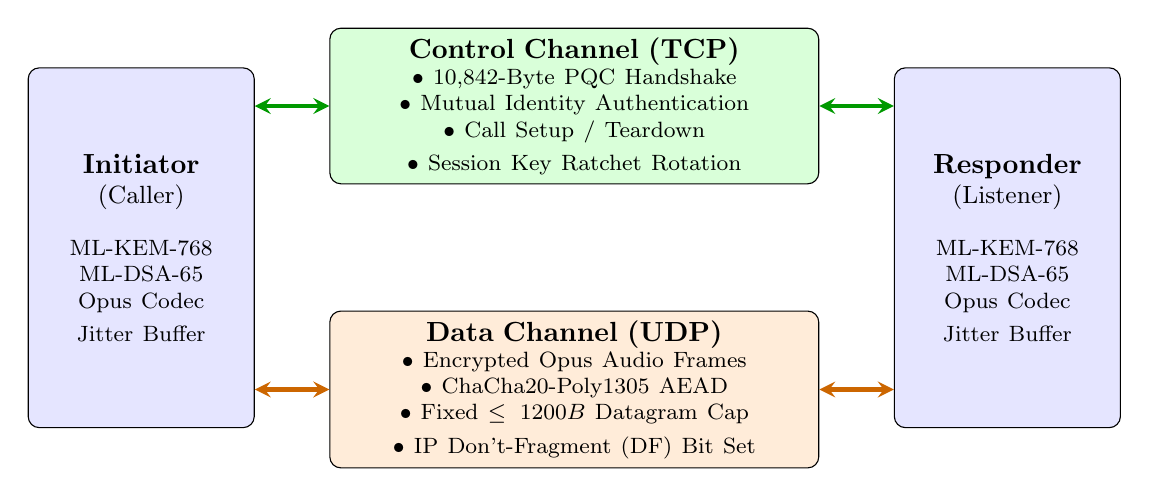
\begin{tikzpicture}[
        every node/.style={align=center},
        peer/.style={rectangle, draw, fill=blue!10, text width=7.5em, align=center, rounded corners, minimum height=13em},
        channel_tcp/.style={rectangle, draw, fill=green!15, text width=17em, align=center, minimum height=4.5em, rounded corners},
        channel_udp/.style={rectangle, draw, fill=orange!15, text width=17em, align=center, minimum height=4.5em, rounded corners},
        link/.style={thick, <->, >=stealth}
    ]
        \node [peer] (init) at (-5.5, 0) {\textbf{Initiator}\\\small (Caller)\\[1em]\footnotesize ML-KEM-768\\ML-DSA-65\\Opus Codec\\Jitter Buffer};
        \node [channel_tcp] (tcp) at (0, 1.8) {\textbf{Control Channel (TCP)}\\\footnotesize $\bullet$ 10,842-Byte PQC Handshake\\$\bullet$ Mutual Identity Authentication\\$\bullet$ Call Setup / Teardown\\$\bullet$ Session Key Ratchet Rotation};
        \node [channel_udp] (udp) at (0, -1.8) {\textbf{Data Channel (UDP)}\\\footnotesize $\bullet$ Encrypted Opus Audio Frames\\$\bullet$ ChaCha20-Poly1305 AEAD\\$\bullet$ Fixed $\le 1200\text{ B}$ Datagram Cap\\$\bullet$ IP Don't-Fragment (DF) Bit Set};
        \node [peer] (resp) at (5.5, 0) {\textbf{Responder}\\\small (Listener)\\[1em]\footnotesize ML-KEM-768\\ML-DSA-65\\Opus Codec\\Jitter Buffer};

        \draw [link, color=green!60!black, line width=1.5pt] (init.east |- tcp.west) -- (tcp.west);
        \draw [link, color=green!60!black, line width=1.5pt] (tcp.east) -- (resp.west |- tcp.east);
        
        \draw [link, color=orange!80!black, line width=1.5pt] (init.east |- udp.west) -- (udp.west);
        \draw [link, color=orange!80!black, line width=1.5pt] (udp.east) -- (resp.west |- udp.east);
    \end{tikzpicture}
    \caption{HPQV Decoupled Dual-Channel Transport Architecture.}
    \label{fig:hpqv_architecture}
\end{figure}

As depicted in Figure \ref{fig:hpqv_architecture}, the two communicating endpoints establish two concurrent connections:
\begin{enumerate}
    \item \textbf{Control Channel (TCP):} A reliable, connection-oriented byte stream that carries the post-quantum cryptographic key exchange, mutual identity verification, signaling messages (\texttt{CALL\_START}, \texttt{CALL\_END}), and forward-secret key ratchet rotations. Because TCP provides transparent byte-stream segmentation and guaranteed delivery via sliding-window retransmissions, the 10,842-byte post-quantum handshake never becomes an IP fragment.
    \item \textbf{Data Channel (UDP):} An unreliable, connectionless datagram path dedicated solely to streaming encrypted Opus voice frames. Datagrams are strictly constrained under a conservative 1,200-byte cap and transmitted with the IPv4 Don't-Fragment (DF) flag asserted. The data plane maintains near-zero queueing latency, delegating frame loss recovery to in-band forward error correction and jitter buffering.
\end{enumerate}

\section{CONTROL CHANNEL SPECIFICATION (TCP)}

\subsection{Framing and Record Layer}
Because TCP is an unformatted byte stream lacking native record boundaries, the HPQV control layer introduces an application-level length-prefixed framing protocol. Every discrete control and cryptographic record transmitted over TCP is encapsulated within a 4-byte big-endian header indicating the payload length:
\begin{equation}
    \text{Record} = \text{Length}\ (4\ \text{bytes, unsigned big-endian integer}) \parallel \text{Payload}\ (L\ \text{bytes})
\end{equation}
The receiver's socket driver executes a bounded reassembly loop (\texttt{\_recvn}), blocking until exactly $L$ bytes have been extracted from the OS kernel buffer. This framing guarantees that variable-length post-quantum messages are parsed unambiguously without risk of TCP stream boundary fragmentation.

\subsection{Control Message Protocol}
Post-handshake session signaling utilizes structured control messages prefixed with a 1-byte message type identifier:
\begin{table}[htbp]
    \centering
    \caption{HPQV Control Plane Message Definitions.}
    \label{tab:control_messages}
    \begin{tabularx}{\textwidth}{>{\raggedright\arraybackslash}p{4.2cm} c >{\raggedright\arraybackslash}p{2.5cm} >{\raggedright\arraybackslash}X}
        \toprule
        \textbf{Identifier} & \textbf{Type Value} & \textbf{Payload} & \textbf{Operational Semantics} \\
        \midrule
        \texttt{MSG\_CALL\_START} & \texttt{0x01} & UDP Port (2B) & Signals readiness to stream voice; exchanges remote UDP port. \\
        \texttt{MSG\_CALL\_END} & \texttt{0x02} & None & Initiates graceful call termination and teardown. \\
        \texttt{MSG\_KEY\_ROTATE} & \texttt{0x03} & None & Instructs peers to ratchet the symmetric session key in lockstep. \\
        \bottomrule
    \end{tabularx}
\end{table}

\section{CRYPTOGRAPHIC HANDSHAKE DESIGN}

\subsection{Cryptographic Primitives and Parameter Selection}
HPQV deploys NIST Security Category 3 lattice-based primitives:
\begin{itemize}
    \item \textbf{Key Encapsulation Mechanism:} ML-KEM-768 \cite{nist_fips203}, operating on rank $k=3$ module lattices over $R_q = \mathbb{Z}_{3329}[X]/(X^{256}+1)$, offering 192 bits of classical security and robust resistance against quantum search algorithms.
    \item \textbf{Digital Signature Algorithm:} ML-DSA-65 \cite{nist_fips204}, parameterized over module lattices with matrix dimensions $(k,\ell) = (6,5)$ and modulus $q=8380417$.
\end{itemize}

\subsection{Handshake Message Structure}
The cryptographic handshake consists of a 2-message exchange: \texttt{HELLO} and \texttt{ACCEPT}.

\subsubsection{1. Initiator HELLO (6,445 Bytes)}
The caller initiates communication by generating an ephemeral ML-KEM-768 keypair $(\text{pk}_{\text{KEM}}, \text{sk}_{\text{KEM}})$. It concatenates this public key with its long-term ML-DSA-65 identity public key $\text{pk}_{\text{DSA}}^{\text{init}}$ and computes a digital signature over both keys using its private identity key $\text{sk}_{\text{DSA}}^{\text{init}}$:
\begin{equation}
    \sigma_{\text{init}} = \text{Sign}_{\text{ML-DSA-65}}(\text{sk}_{\text{DSA}}^{\text{init}}, \text{pk}_{\text{KEM}} \parallel \text{pk}_{\text{DSA}}^{\text{init}})
\end{equation}
The formatted \texttt{HELLO} message wire layout is:
\begin{equation}
    \text{HELLO} = \text{Version}\ (1\text{B}) \parallel \text{pk}_{\text{KEM}}\ (1184\text{B}) \parallel \text{pk}_{\text{DSA}}^{\text{init}}\ (1952\text{B}) \parallel \sigma_{\text{init}}\ (3309\text{B})
\end{equation}
Total byte length $= 1 + 1184 + 1952 + 3309 = \mathbf{6,445\ \text{bytes}}$.

\subsubsection{2. Responder ACCEPT (4,397 Bytes)}
Upon receiving \texttt{HELLO}, the responder extracts the public keys and verifies the initiator's identity against its pinned trust store. If valid, the responder encapsulates a 256-bit shared secret using $\text{pk}_{\text{KEM}}$:
\begin{equation}
    (\text{ct}_{\text{KEM}}, K_{\text{shared}}) = \text{Encap}_{\text{ML-KEM-768}}(\text{pk}_{\text{KEM}})
\end{equation}
The responder authenticates the exchange by computing its own ML-DSA-65 signature over the transcript:
\begin{equation}
    \sigma_{\text{resp}} = \text{Sign}_{\text{ML-DSA-65}}(\text{sk}_{\text{DSA}}^{\text{resp}}, \text{pk}_{\text{KEM}} \parallel \text{ct}_{\text{KEM}})
\end{equation}
The formatted \texttt{ACCEPT} wire layout is:
\begin{equation}
    \text{ACCEPT} = \text{Version}\ (1\text{B}) \parallel \text{ct}_{\text{KEM}}\ (1088\text{B}) \parallel \sigma_{\text{resp}}\ (3309\text{B})
\end{equation}
Total byte length $= 1 + 1088 + 3309 = \mathbf{4,397\ \text{bytes}}$. Combined handshake total is $\mathbf{10,842\ \text{bytes}}$.

\begin{figure}[htbp]
    \centering
    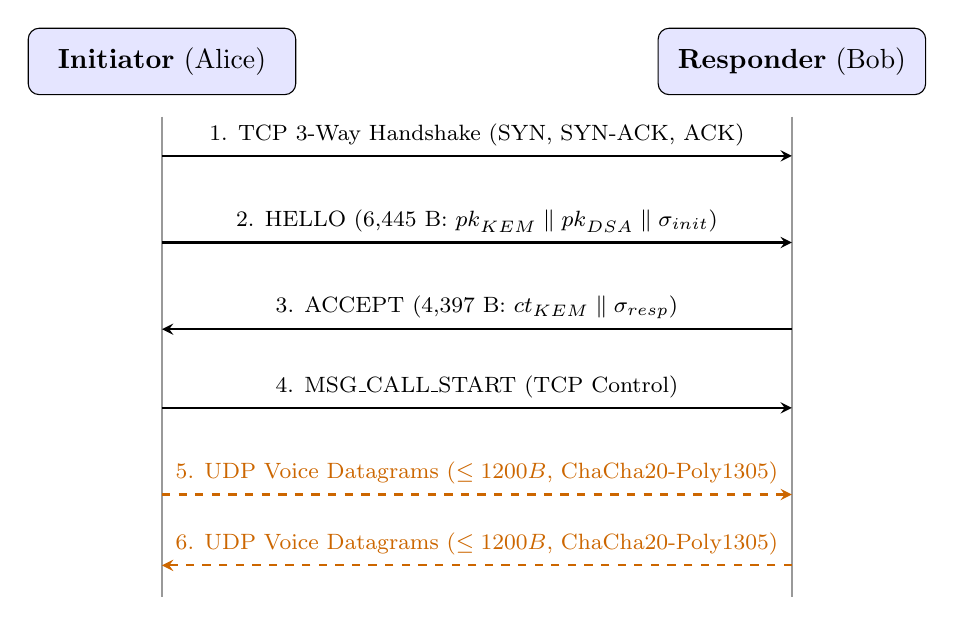
\begin{tikzpicture}[
        every node/.style={align=center},
        entity/.style={rectangle, draw, fill=blue!10, text width=9em, align=center, minimum height=2.4em, rounded corners},
        msg/.style={thick, ->, >=stealth},
        mediamattr/.style={thick, ->, >=stealth, dashed, color=orange!80!black}
    ]
        \node [entity] (init) at (-4, 5.0) {\textbf{Initiator} (Alice)};
        \node [entity] (resp) at (4, 5.0) {\textbf{Responder} (Bob)};
        
        \draw [thick, black!40] (-4, 4.3) -- (-4, -1.8);
        \draw [thick, black!40] (4, 4.3) -- (4, -1.8);

        \draw [msg] (-4, 3.8) -- node[above]{\footnotesize 1. TCP 3-Way Handshake (SYN, SYN-ACK, ACK)} (4, 3.8);
        \draw [msg] (-4, 2.7) -- node[above]{\footnotesize 2. HELLO (6,445 B: $\text{pk}_{\text{KEM}} \parallel \text{pk}_{\text{DSA}} \parallel \sigma_{\text{init}}$)} (4, 2.7);
        \draw [msg] (4, 1.6) -- node[above]{\footnotesize 3. ACCEPT (4,397 B: $\text{ct}_{\text{KEM}} \parallel \sigma_{\text{resp}}$)} (-4, 1.6);
        \draw [msg] (-4, 0.6) -- node[above]{\footnotesize 4. MSG\_CALL\_START (TCP Control)} (4, 0.6);
        
        \draw [mediamattr] (-4, -0.5) -- node[above]{\footnotesize 5. UDP Voice Datagrams ($\le 1200\text{ B}$, ChaCha20-Poly1305)} (4, -0.5);
        \draw [mediamattr] (4, -1.4) -- node[above]{\footnotesize 6. UDP Voice Datagrams ($\le 1200\text{ B}$, ChaCha20-Poly1305)} (-4, -1.4);
    \end{tikzpicture}
    \caption{Sequential Execution Flow of the HPQV Protocol.}
    \label{fig:handshake_sequence}
\end{figure}

\section{MUTUAL AUTHENTICATION AND TRANSCRIPT BINDING}

\subsection{Vulnerability Analysis of Unilateral Authentication}
During initial development, the handshake prototype implemented unilateral authentication: while the initiator authenticated its identity via $\sigma_{\text{init}}$, the responder's \texttt{ACCEPT} message contained only the raw ciphertext $\text{ct}_{\text{KEM}}$.

As documented in Architecture Decision Record 0002 (ADR-0002), this unilateral design possessed a severe Man-in-the-Middle (MITM) vulnerability. An active network adversary $\mathcal{A}$ on the TCP control path could observe the unauthenticated \texttt{ACCEPT} message, discard it, and substitute its own encapsulated ciphertext $\text{ct}'_{\mathcal{A}}$ derived from the initiator's public $\text{pk}_{\text{KEM}}$. Because the initiator lacked cryptographic proof that the ciphertext originated from the intended peer, it would decapsulate $\text{ct}'_{\mathcal{A}}$, establishing a shared key with the adversary rather than the legitimate responder.

\subsection{Cryptographic Transcript Binding (ADR-0002)}
To eliminate MITM attacks, HPQV mandates mutual authentication. The responder must possess an out-of-band pinned identity key $\text{pk}_{\text{DSA}}^{\text{resp}}$. In the \texttt{ACCEPT} record, the responder binds the cryptographic transcript by signing the exact concatenation of the initiator's public key and the resulting ciphertext:
\begin{equation}
    \mathcal{M}_{\text{transcript}} = \text{pk}_{\text{KEM}} \parallel \text{ct}_{\text{KEM}}
\end{equation}
Prior to executing decapsulation, the initiator verifies $\sigma_{\text{resp}}$ against the trusted $\text{pk}_{\text{DSA}}^{\text{resp}}$:
\begin{equation}
    \text{Verify}_{\text{ML-DSA-65}}(\text{pk}_{\text{DSA}}^{\text{resp}}, \mathcal{M}_{\text{transcript}}, \sigma_{\text{resp}}) \stackrel{?}{=} \text{True}
\end{equation}
If verification fails, the connection aborts immediately with an \texttt{unpinned identity} or \texttt{bad signature} exception. This transcript binding guarantees that an adversary cannot alter or substitute the encapsulation.

\section{KEY DERIVATION AND DIRECTIONAL NONCE SEPARATION}

\subsection{HKDF Expansion}
Following successful decapsulation, both peers possess an identical 256-bit post-quantum shared secret $K_{\text{shared}}$. HPQV expands this secret using the HMAC-based Key Derivation Function (HKDF-SHA256, RFC 5869) \cite{rfc5869}:
\begin{equation}
    \text{OKM} = \text{HKDF-Expand}(\text{PRK} = K_{\text{shared}}, \text{info} = \text{b"hpqv v1"}, \text{length} = 40)
\end{equation}
The 40-byte output keying material ($\text{OKM}$) is sliced into three distinct cryptographic values:
\begin{equation}
    K_{\text{voice}} = \text{OKM}[0:32],\quad \text{Prefix}_{I \to R} = \text{OKM}[32:36],\quad \text{Prefix}_{R \to I} = \text{OKM}[36:40]
\end{equation}
\begin{itemize}
    \item $K_{\text{voice}}$: A 256-bit symmetric key dedicated to data-plane ChaCha20-Poly1305 encryption.
    \item $\text{Prefix}_{I \to R}$: A 4-byte nonce prefix for voice packets traveling from Initiator to Responder.
    \item $\text{Prefix}_{R \to I}$: A 4-byte nonce prefix for voice packets traveling from Responder to Initiator.
\end{itemize}

\subsection{Elimination of Nonce Reuse Vulnerabilities}
The construction of distinct directional nonce prefixes solves a critical cryptographic hazard. ChaCha20-Poly1305 (RFC 7539) is an Authenticated Encryption with Associated Data (AEAD) cipher requiring a 96-bit (12-byte) nonce \cite{rfc7539}. It is a well-established cryptographic fact that reusing a single (Key, Nonce) pair under ChaCha20-Poly1305 completely destroys authenticity: an adversary observing two ciphertexts encrypted under identical nonces can XOR the ciphertexts to recover plaintext differences and compute the underlying Poly1305 authenticator key, permitting undetected ciphertext forgery.

In a full-duplex VoIP session, both endpoints begin streaming audio simultaneously, each initializing their sequence counter at zero ($\text{seq} = 0$). If both directions utilized a shared nonce prefix, the initiator's first packet and the responder's first packet would possess identical 12-byte nonces:
\begin{equation}
    \text{Nonce}_{I \to R}(0) = \text{Prefix} \parallel 0 = \text{Nonce}_{R \to I}(0)
\end{equation}
By deriving two mathematically independent 4-byte prefixes from HKDF and enforcing:
\begin{align}
    \text{Nonce}_{I \to R}(\text{seq}) &= \text{Prefix}_{I \to R}\ (4\text{B}) \parallel \text{seq}\ (8\text{B, big-endian}) \\
    \text{Nonce}_{R \to I}(\text{seq}) &= \text{Prefix}_{R \to I}\ (4\text{B}) \parallel \text{seq}\ (8\text{B, big-endian})
\end{align}
HPQV strictly partitions the nonce spaces, ensuring that identical nonces are never generated across the lifetime of the session.

\section{DYNAMIC KEY ROTATION AND RATCHETING}
To maintain forward secrecy throughout long-duration calls, HPQV implements an HKDF-based key ratchet mechanism. Either endpoint can trigger key rotation by dispatching an authenticated \texttt{MSG\_KEY\_ROTATE} control record over TCP.

Both endpoints ratchet their symmetric state deterministically:
\begin{equation}
    \text{OKM}_{\text{next}} = \text{HKDF-Expand}(\text{PRK} = K_{\text{current}}, \text{info} = \text{b"hpqv rotate v1"}, \text{length} = 40)
\end{equation}
Extracting:
\begin{equation}
    K_{\text{new}} = \text{OKM}_{\text{next}}[0:32],\quad P_0 = \text{OKM}_{\text{next}}[32:36],\quad P_1 = \text{OKM}_{\text{next}}[36:40]
\end{equation}
To ensure that peers maintain mirrored send and receive prefix assignments without ambiguity, prefixes are mapped via a canonical lexicographic comparison:
\begin{equation}
    (\text{SendPrefix}_{\text{new}}, \text{RecvPrefix}_{\text{new}}) = 
    \begin{cases}
        (P_0, P_1), & \text{if } \text{SendPrefix}_{\text{current}} < \text{RecvPrefix}_{\text{current}} \\
        (P_1, P_0), & \text{otherwise}
    \end{cases}
\end{equation}
Upon ratcheting, packet sequence numbers reset to zero ($\text{seq} = 0$), and the old session key is overwritten in memory.

\section{DATA CHANNEL SPECIFICATION (UDP)}

\subsection{Voice Datagram Header and AEAD Framing}
The HPQV voice datagram layout is engineered for minimal framing overhead while providing complete packet authenticity:

\begin{figure}[htbp]
    \centering
    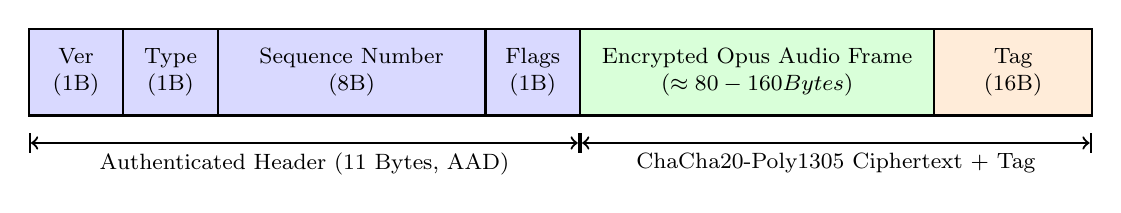
\begin{tikzpicture}[
        every node/.style={align=center, font=\footnotesize}
    ]
        \draw[thick, fill=blue!15] (0,0) rectangle (1.2,1.1) node[pos=.5]{Ver\\(1B)};
        \draw[thick, fill=blue!15] (1.2,0) rectangle (2.4,1.1) node[pos=.5]{Type\\(1B)};
        \draw[thick, fill=blue!15] (2.4,0) rectangle (5.8,1.1) node[pos=.5]{Sequence Number\\(8B)};
        \draw[thick, fill=blue!15] (5.8,0) rectangle (7.0,1.1) node[pos=.5]{Flags\\(1B)};
        \draw[thick, fill=green!15] (7.0,0) rectangle (11.5,1.1) node[pos=.5]{Encrypted Opus Audio Frame\\($\approx 80-160\text{ Bytes}$)};
        \draw[thick, fill=orange!15] (11.5,0) rectangle (13.5,1.1) node[pos=.5]{Tag\\(16B)};

        % Dimension lines below boxes
        \draw[thick, |<->|] (0,-0.35) -- (7.0,-0.35) node[midway, below]{Authenticated Header (11 Bytes, AAD)};
        \draw[thick, |<->|] (7.0,-0.35) -- (13.5,-0.35) node[midway, below]{ChaCha20-Poly1305 Ciphertext + Tag};
    \end{tikzpicture}
    \caption{HPQV Data-Plane Voice Datagram Layout.}
    \label{fig:packet_layout}
\end{figure}

As shown in Figure \ref{fig:packet_layout}, the unencrypted header occupies exactly 11 bytes:
\begin{equation}
    \text{Header} = \text{Ver}\ (1\text{B}) \parallel \text{Type}\ (1\text{B}) \parallel \text{SeqNum}\ (8\text{B}) \parallel \text{Flags}\ (1\text{B})
\end{equation}
This 11-byte header is supplied as Associated Authenticated Data (AAD) to the ChaCha20-Poly1305 cipher. Any tampering with sequence numbers, packet types, or flags causes decryption to fail.

\subsection{Enforced Datagram Invariant and DF Flag}
To ensure that data-plane traffic never experiences IP-layer fragmentation under any network condition, HPQV implements a dual-layer architectural invariant:
\begin{enumerate}
    \item \textbf{Application-Level Sizing Guard:} The datagram serialization function (\texttt{packet.seal}) explicitly evaluates the assembled packet size. If the length exceeds 1,200 bytes, the function raises an immediate runtime exception:
    \begin{equation}
        \text{Length}(\text{Header} \parallel \text{Ciphertext} \parallel \text{Tag}) \le 1200\ \text{bytes}
    \end{equation}
    Because standard 20 ms Opus frames compress speech to 80--160 bytes, the total datagram size typically spans 110--190 bytes—well below the 1,200-byte threshold.
    \item \textbf{Kernel-Level Don't-Fragment Bit:} The underlying UDP socket is initialized with explicit operating system socket options setting the Don't-Fragment (DF) flag (\texttt{IP\_MTU\_DISCOVER} with \texttt{IP\_PMTUDISC\_DO} on Linux; \texttt{IP\_DONTFRAGMENT} on Windows). If an anomalous packet exceeds path MTU, the OS drops the packet locally rather than fragmenting it.
\end{enumerate}

\section{AUDIO PROCESSING AND RESILIENCE PIPELINE}

\subsection{Opus Codec Integration}
HPQV processes wideband audio at 48,000 Hz (48 kHz) mono with 16-bit linear PCM. Audio frames are grouped into 20 ms chunks:
\begin{equation}
    \text{Frame Samples} = 48000 \times 0.020 = 960\ \text{samples} = 1,920\ \text{bytes PCM}
\end{equation}
The Opus encoder operates in \texttt{APPLICATION\_VOIP} mode with in-band Forward Error Correction (LBRR) active.

\subsection{Jitter Buffer Architecture}
Network packet arrival over UDP is non-deterministic. To resolve packet reordering, delay jitter, and duplicate deliveries, HPQV incorporates a fixed-depth min-heap jitter buffer (depth $D=3$ frames, corresponding to 60 ms buffer depth).
\begin{algorithm}[htbp]
\caption{HPQV Jitter Buffer Ingestion and Extraction}
\label{alg:jitter_buffer}
\begin{algorithmic}[1]
\Require Sequence number $s$, Audio payload $f$, State: $\text{Heap } H$, $\text{SeenSet } S$, $\text{LastSeq } L$, Depth $D$
\Procedure{Push}{$s, f$}
    \If{$s \le L$ \textbf{or} $s \in S$}
        \State \Return \Comment{Discard duplicate or stale packet}
    \EndIf
    \State $S \gets S \cup \{s\}$
    \State $\text{HeapPush}(H, (s, f))$
\EndProcedure
\Procedure{Pop}{}
    \If{$\text{Length}(H) < D$}
        \State \Return $\text{None}$ \Comment{Buffering to absorb network jitter}
    \EndIf
    \State $(s_{\text{min}}, f_{\text{min}}) \gets \text{HeapPop}(H)$
    \State $S \gets S \setminus \{s_{\text{min}}\}$
    \State $L \gets s_{\text{min}}$
    \State \Return $f_{\text{min}}$
\EndProcedure
\end{algorithmic}
\end{algorithm}
As detailed in Algorithm \ref{alg:jitter_buffer}, incoming frames are inserted into min-heap $H$. Packets with sequence numbers older than the last popped packet ($s \le L$) are dropped as expired. Only when buffer occupancy reaches depth $D$ does \texttt{Pop()} extract the lowest sequence number, ensuring perfectly ordered playout.


% Chapter 4: Implementation Details & Software Architecture
\chapter{IMPLEMENTATION DETAILS AND SOFTWARE ARCHITECTURE}

\section{DEVELOPMENT ENVIRONMENT AND DEPENDENCY STACK}
The reference implementation of the HPQV protocol is engineered as a clean, modular Python 3.11 package comprising approximately 1,100 lines of core protocol code (excluding automated test suites and evaluation drivers). The software stack leverages high-performance C libraries accessed via Foreign Function Interfaces (FFI) and ctypes:

\begin{table}[htbp]
    \centering
    \caption{HPQV Implementation Technology Stack and Dependencies.}
    \label{tab:tech_stack}
    \begin{tabularx}{\textwidth}{>{\raggedright\arraybackslash}p{2.6cm} >{\raggedright\arraybackslash}p{3.2cm} c >{\raggedright\arraybackslash}X}
        \toprule
        \textbf{Component} & \textbf{Library / Package} & \textbf{Version} & \textbf{Architectural Responsibility} \\
        \midrule
        Runtime & CPython & 3.11.9 & Pinned execution environment managed via \texttt{uv}. \\
        Post-Quantum Crypto & \texttt{liboqs} / \texttt{liboqs-python} & 0.10.0 & C-based primitives for ML-KEM-768 and ML-DSA-65. \\
        Symmetric Crypto & \texttt{cryptography} (PyCA) & 42.0.5 & ChaCha20-Poly1305 AEAD and HKDF-SHA256 expansion. \\
        Audio Codec & \texttt{libopus} / \texttt{opuslib} & 3.0.1 & Low-latency speech compression and in-band FEC. \\
        Audio I/O & \texttt{sounddevice} / PortAudio & 0.4.6 & Full-duplex microphone capture and speaker rendering. \\
        User Interface & \texttt{tkinter} & Stdlib & Desktop graphical interface with live loss slider. \\
        Testing Harness & \texttt{pytest} & 8.1.1 & Automated unit, integration, and security verification. \\
        \bottomrule
    \end{tabularx}
\end{table}

\section{RUNTIME ANOMALIES AND SYSTEM WORKAROUNDS}
During the engineering of the prototype, several non-trivial cross-platform runtime bugs were identified and resolved:

\subsection{Opuslib In-Band FEC Binding Defect}
In \texttt{opuslib 3.0.1}, the Python property setter \texttt{inband\_fec} contains an upstream ctypes binding defect: the wrapper function fails to forward the integer boolean argument to the underlying C function, rendering \texttt{encoder.inband\_fec = True} a silent no-op. To ensure that Forward Error Correction (LBRR) is properly activated in the C runtime, \texttt{hpqv.audio} bypasses the property setter and invokes the native encoder control routine directly:
\begin{lstlisting}[language=Python]
# Workaround for upstream ctypes binding defect in opuslib 3.0.1
opuslib.api.encoder.encoder_ctl(
    self.enc.encoder_state, 
    opuslib.api.ctl.set_inband_fec, 
    1
)
self.enc.packet_loss_perc = 10
\end{lstlisting}

\subsection{Dynamic Linker Resolution under macOS SIP}
On macOS systems, System Integrity Protection (SIP) scrubs dynamic library search paths for spawned subprocesses. Consequently, \texttt{ctypes.util.find\_library('opus')} returns \texttt{None}, preventing \texttt{opuslib} from discovering Homebrew-installed shared libraries in \texttt{/opt/homebrew/lib}. This was resolved by injecting the fallback linker variable \texttt{DYLD\_FALLBACK\_LIBRARY\_PATH=/opt/homebrew/lib} across test configurations and CLI runners.

\subsection{Cross-Platform Socket Configuration for DF Bit}
Setting the IP Don't-Fragment bit requires distinct low-level operating system socket options across UNIX and Windows kernels. HPQV encapsulates this in \texttt{hpqv.udp}:
\begin{lstlisting}[language=Python]
import socket, sys

def make_udp_socket():
    sock = socket.socket(socket.AF_INET, socket.SOCK_DGRAM)
    if sys.platform.startswith("linux"):
        # IP_MTU_DISCOVER with IP_PMTUDISC_DO (sets DF bit)
        sock.setsockopt(socket.IPPROTO_IP, 10, 2)
    elif sys.platform == "win32":
        # IP_DONTFRAGMENT flag
        sock.setsockopt(socket.IPPROTO_IP, 14, 1)
    return sock
\end{lstlisting}

\section{CORE SYSTEM MODULE BREAKDOWN}
The codebase is partitioned into eight focused modules within \texttt{src/hpqv/}:

\begin{figure}[htbp]
    \centering
    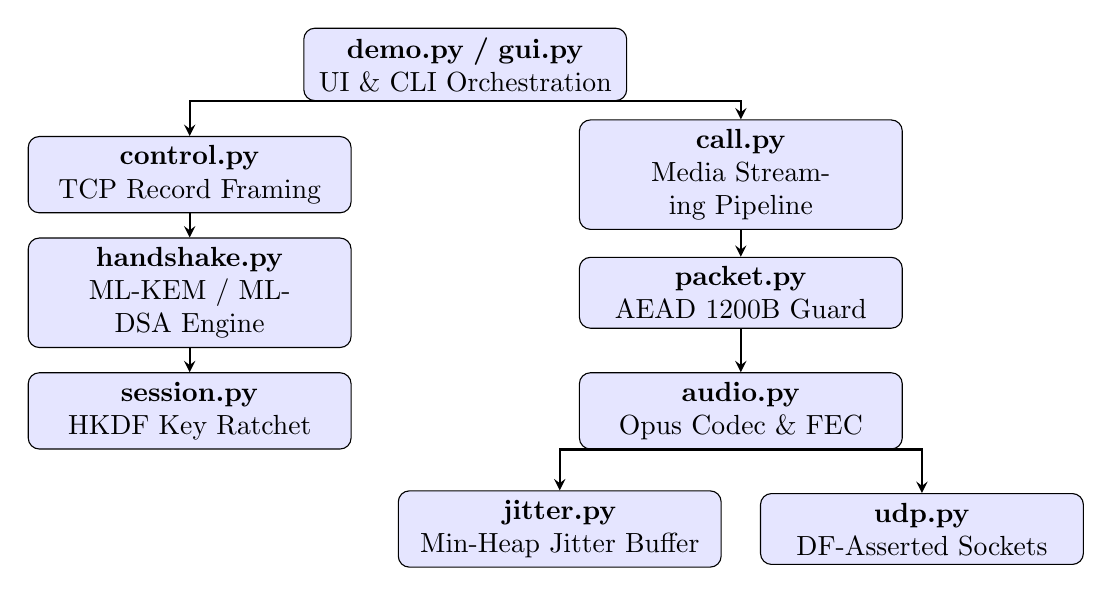
\begin{tikzpicture}[
        every node/.style={align=center},
        mod/.style={rectangle, draw, fill=blue!10, text width=11em, align=center, rounded corners, minimum height=2.4em},
        conn/.style={thick, ->, >=stealth}
    ]
        \node [mod] (demo) at (0, 4.0) {\textbf{demo.py / gui.py}\\UI \& CLI Orchestration};
        
        \node [mod] (ctrl) at (-3.5, 2.6) {\textbf{control.py}\\TCP Record Framing};
        \node [mod] (call) at (3.5, 2.6) {\textbf{call.py}\\Media Streaming Pipeline};
        
        \node [mod] (hs) at (-3.5, 1.1) {\textbf{handshake.py}\\ML-KEM / ML-DSA Engine};
        \node [mod] (sess) at (-3.5, -0.4) {\textbf{session.py}\\HKDF Key Ratchet};
        
        \node [mod] (pkt) at (3.5, 1.1) {\textbf{packet.py}\\AEAD 1200B Guard};
        \node [mod] (aud) at (3.5, -0.4) {\textbf{audio.py}\\Opus Codec \& FEC};
        \node [mod] (jit) at (1.2, -1.9) {\textbf{jitter.py}\\Min-Heap Jitter Buffer};
        \node [mod] (udp) at (5.8, -1.9) {\textbf{udp.py}\\DF-Asserted Sockets};

        \draw [conn] (demo.south) -| (ctrl.north);
        \draw [conn] (demo.south) -| (call.north);
        \draw [conn] (ctrl) -- (hs);
        \draw [conn] (hs) -- (sess);
        \draw [conn] (call) -- (pkt);
        \draw [conn] (pkt) -- (aud);
        \draw [conn] (aud.south) -| (jit.north);
        \draw [conn] (aud.south) -| (udp.north);
    \end{tikzpicture}
    \caption{Module Interaction and Dependency Architecture of HPQV.}
    \label{fig:module_architecture}
\end{figure}

\subsection{Cryptographic Handshake Engine (\texttt{handshake.py})}
Implements the core post-quantum primitives using \texttt{liboqs-python}:
\begin{itemize}
    \item \texttt{make\_identity()}: Generates a long-term ML-DSA-65 identity keypair $(\text{pk}_{\text{DSA}}, \text{sk}_{\text{DSA}})$.
    \item \texttt{build\_hello(sig\_pub, sig\_secret)}: Generates an ephemeral ML-KEM-768 keypair, signs $\text{pk}_{\text{KEM}} \parallel \text{pk}_{\text{DSA}}$, and packs the 6,445-byte \texttt{HELLO} record.
    \item \texttt{accept\_hello(hello, trusted\_sig\_pub, sig\_secret)}: Parses \texttt{HELLO}, asserts pinned identity matching, verifies the caller's signature, encapsulates a 256-bit shared secret, signs $\text{pk}_{\text{KEM}} \parallel \text{ct}_{\text{KEM}}$, derives keys via HKDF, and returns the 4,397-byte \texttt{ACCEPT} record.
    \item \texttt{finish(accept, kem, kem\_pub, trusted\_sig\_pub)}: Verifies the responder's signature against the pinned identity, decapsulates the shared secret, and derives symmetric session keys.
\end{itemize}

\subsection{Control Framing Driver (\texttt{control.py})}
Provides reliable length-prefixed I/O over TCP sockets:
\begin{lstlisting}[language=Python]
import struct

def send_record(sock, payload: bytes) -> None:
    sock.sendall(struct.pack(">I", len(payload)) + payload)

def _recvn(sock, n: int) -> bytes:
    buf = b""
    while len(buf) < n:
        chunk = sock.recv(n - len(buf))
        if not chunk:
            raise ConnectionError("peer closed")
        buf += chunk
    return buf

def recv_record(sock) -> bytes:
    (length,) = struct.unpack(">I", _recvn(sock, 4))
    return _recvn(sock, length)
\end{lstlisting}

\subsection{Packet Serialization and AEAD Sealing (\texttt{packet.py})}
Constructs and validates voice datagrams:
\begin{lstlisting}[language=Python]
import struct
from cryptography.hazmat.primitives.ciphers.aead import ChaCha20Poly1305

MAX_DATAGRAM = 1200
VERSION, TYPE_VOICE = 1, 1

def _header(seq: int, flags: int) -> bytes:
    return struct.pack(">BBQB", VERSION, TYPE_VOICE, seq, flags)

def seal(key, nonce_prefix, seq, opus_frame, flags=0):
    header = _header(seq, flags)
    nonce = nonce_prefix + struct.pack(">Q", seq)
    ct = ChaCha20Poly1305(key).encrypt(nonce, opus_frame, header)
    dg = header + ct
    if len(dg) > MAX_DATAGRAM:
        raise ValueError(f"datagram {len(dg)} > {MAX_DATAGRAM}")
    return dg
\end{lstlisting}

\section{DESKTOP DEMONSTRATION AND GRAPHICAL USER INTERFACE}

\subsection{Command-Line Interface (\texttt{demo.py})}
The system provides a complete CLI interface supporting three primary commands:
\begin{enumerate}
    \item \texttt{keygen --out identity.json}: Generates paired ML-DSA-65 identity keys for caller and listener.
    \item \texttt{listen --port 9000 --identity-file identity.json}: Runs the answering responder daemon.
    \item \texttt{call <IP:port> --identity-file identity.json}: Initiates a secure call to the remote endpoint.
\end{enumerate}
Audio frames can be sourced live from the microphone via \texttt{sounddevice} or read from pre-recorded PCM WAV files with 20 ms frame pacing.

\subsection{Interactive Graphical User Interface (\texttt{gui.py})}
To facilitate live peer evaluations, HPQV includes an interactive Tkinter graphical interface. The GUI features:
\begin{itemize}
    \item \textbf{Asynchronous Threading Architecture:} All socket I/O and cryptographic operations run on dedicated background worker threads. A thread-safe \texttt{queue.Queue} transmits status events to the main thread, polled via \texttt{root.after(200, self.\_poll)} to prevent GUI freezing.
    \item \textbf{Live Audio VU Meters:} Progress bars monitor outbound and inbound RMS audio energy in real time.
    \item \textbf{Dynamic In-Call Packet Loss Slider:} Allows an operator to adjust synthetic packet drop probabilities (from 0\% to 50\%) in real time during an ongoing live call. The audience can directly hear speech degrade and recover as the slider is manipulated, while the dropped packet telemetry counter updates live.
\end{itemize}

\section{AUTOMATED TESTING AND VERIFICATION SUITE}
The implementation is validated by a rigorous test suite comprising 53 automated unit and integration tests executing under \texttt{pytest}.

\begin{table}[htbp]
    \centering
    \caption{Distribution and Verification Targets of the 53-Case Automated Test Suite.}
    \label{tab:test_suite}
    \small
    \begin{tabularx}{\textwidth}{>{\raggedright\arraybackslash}p{4.2cm} c >{\raggedright\arraybackslash}X}
        \toprule
        \textbf{Test Module} & \textbf{Count} & \textbf{Protected Invariants and Behavioral Verification} \\
        \midrule
        \texttt{test\_handshake.py} & 4 & Key agreement derivation, mutual auth, rejection of forged ACCEPT or tampered ciphertext. \\
        \texttt{test\_control.py} & 3 & Framing record round-trip, TCP control state machine, signaling message delivery. \\
        \texttt{test\_session.py} & 2 & Lockstep HKDF key ratcheting, verification of forward secrecy and key modification. \\
        \texttt{test\_packet.py} & 3 & AEAD round-trip, sequence enforcement, strict rejection of datagrams exceeding 1,200 bytes. \\
        \texttt{test\_jitter.py} & 2 & Packet reordering via min-heap, duplicate suppression, late packet drop, clean buffer flush. \\
        \texttt{test\_audio.py} & 1 & Opus 48 kHz / 20 ms encode-decode round-trip fidelity. \\
        \texttt{test\_udp.py} & 1 & Platform-specific socket creation and DF bit assertion. \\
        \texttt{test\_call.py} & 2 & Localhost end-to-end call, verification of directional nonce prefix divergence. \\
        \texttt{test\_loss\_control.py} & 2 & Dynamic loss parameter modification during active audio streaming. \\
        \texttt{eval/test\_mos.py} & 5 & ITU-T G.107 E-model monotonicity, clamping, and continuity at knee boundary. \\
        \texttt{eval/test\_fec\_recovery.py} & 3 & Opus in-band FEC frame recovery and monotonic SNR degradation under loss. \\
        \texttt{eval/test\_handshake\_survival.py} & 3 & Empirical failure of fragmented UDP handshake vs. 100\% survival of hybrid TCP. \\
        \texttt{eval/test\_capture.py} & 2 & Accurate detection of IP fragments in PCAP traces using TShark filters. \\
        \texttt{eval/test\_baselines.py} & 2 & Verification that naive UDP creates 8 fragments while TCP baseline operates cleanly. \\
        \texttt{eval/test\_pqc\_cost.py} & 3 & Calibration of ML-KEM-768 / ML-DSA-65 byte sizes and CPU execution timings. \\
        \texttt{eval/test\_ns3\_smoke.py} & 2 & Compilation and execution integrity of the NS-3 C++ simulation model. \\
        \texttt{Miscellaneous} & 13 & Smoke tests, table renderer sync tests, NetEm teardown cleanup tests. \\
        \midrule
        \textbf{Total Test Cases} & \textbf{53} & \textbf{100\% Pass in Linux Container (38 pass, 15 clean skips on macOS).} \\
        \bottomrule
    \end{tabularx}
\end{table}


% Chapter 5: Experimental Methodology and Setup
\chapter{EXPERIMENTAL METHODOLOGY AND SETUP}

\section{EVALUATION METHODOLOGY AND STRATEGY}
A central principle of this research is empirical honesty: claims regarding network protocol performance must be established through physical measurement of real network packets rather than theoretical speculation or ungrounded simulations. To achieve both realism and comparative breadth, our evaluation is organized across three complementary tiers:

\begin{figure}[htbp]
    \centering
    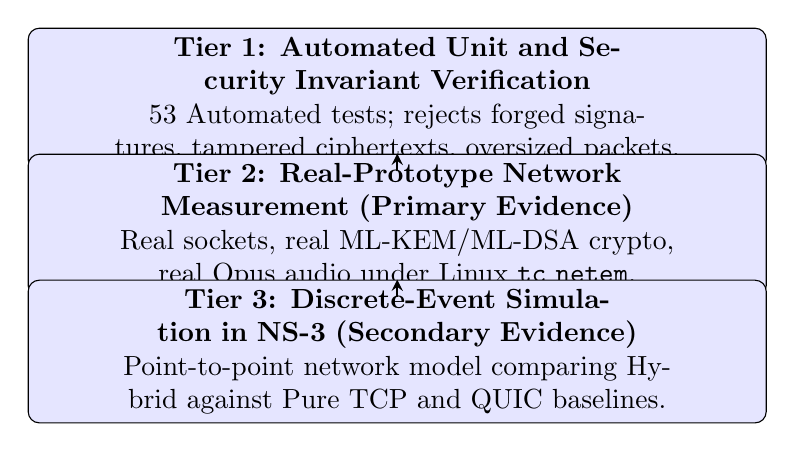
\begin{tikzpicture}[
        every node/.style={align=center},
        tier/.style={rectangle, draw, fill=blue!10, text width=26em, align=center, rounded corners, minimum height=3em},
        conn/.style={thick, ->, >=stealth}
    ]
        \node [tier] (l1) at (0, 3.2) {\textbf{Tier 1: Automated Unit and Security Invariant Verification}\\53 Automated tests; rejects forged signatures, tampered ciphertexts, oversized packets.};
        \node [tier] (l2) at (0, 1.6) {\textbf{Tier 2: Real-Prototype Network Measurement (Primary Evidence)}\\Real sockets, real ML-KEM/ML-DSA crypto, real Opus audio under Linux \texttt{tc netem}.};
        \node [tier] (l3) at (0, 0.0) {\textbf{Tier 3: Discrete-Event Simulation in NS-3 (Secondary Evidence)}\\Point-to-point network model comparing Hybrid against Pure TCP and QUIC baselines.};

        \draw [conn] (l1) -- (l2);
        \draw [conn] (l2) -- (l3);
    \end{tikzpicture}
    \caption{Three-Tiered Evaluation Hierarchy of the HPQV Protocol.}
    \label{fig:evaluation_tiers}
\end{figure}

As documented in Architecture Decision Record 0001 (ADR-0001), the real userspace prototype under Linux Traffic Control (\texttt{tc netem}) serves as the \textbf{primary empirical evidence}. This architectural decision was governed by three physical factors:
\begin{enumerate}
    \item \textbf{Absence of Native PQC in Simulators:} Network simulators such as NS-3 cannot execute cryptographic libraries natively without legacy extensions (such as Direct Code Execution), which are unmaintained and fragile.
    \item \textbf{Realistic Codec and Perceptual Processing:} Simulators treat media as synthetic fixed-rate bit streams. Evaluating speech intelligibility requires running the actual Opus encoder, decoder, and in-band forward error correction routines over real PCM audio.
    \item \textbf{Physical IP Fragmentation Semantics:} Proving that a transport is fragmentation-free requires observing the operating system's IP layer—specifically verifying the absence of IP header More-Fragments (MF) flags and non-zero fragment offsets in raw packet captures.
\end{enumerate}

Simultaneously, as documented in ADR-0003, NS-3 was incorporated as a \textbf{secondary, corroborating model}. NS-3 allows evaluating wide-area propagation delays and benchmarking against protocols (such as QUIC) that cannot be easily embedded into the Python prototype.

\section{REPRODUCIBLE CONTAINERIZED TESTBED}
Linux kernel traffic control (\texttt{tc netem}) and NS-3 do not execute natively on macOS or bare-metal Windows environments. To ensure absolute reproducibility, the complete evaluation suite is packaged within an isolated Ubuntu 24.04 Docker container (\texttt{eval/Dockerfile}) equipped with Python 3.11, \texttt{liboqs}, \texttt{libopus}, \texttt{iproute2}, \texttt{tshark}, and NS-3 version 3.41.

\subsection{The Critical Loopback MTU Discovery}
During early experimentation, a perplexing empirical anomaly was discovered: when running oversized naive UDP handshakes inside Docker containers, packet captures reported zero IP fragments, falsely suggesting that fragmentation was not occurring.

Investigation into container network namespaces revealed that Docker's default loopback interface (\texttt{lo}) is configured with an MTU of \textbf{65,536 bytes} ($64\text{ KB}$). Under a 64 KB MTU, a 10,842-byte handshake datagram fits easily within a single unfragmented frame. Without correcting this parameter, any comparison of IP fragmentation silently measures nothing.

To eliminate this artifact, every evaluation runner within our harness explicitly pins the loopback MTU to the standard Ethernet threshold of 1,500 bytes prior to benchmarking, restoring standard configuration upon teardown:
\begin{lstlisting}[language=bash]
# Pin loopback MTU to realistic Ethernet link capacity
ip link set dev lo mtu 1500
\end{lstlisting}

\section{TRACK 2: REAL-PROTOTYPE EXPERIMENTAL SETUP}

\subsection{Impairment Injection via Linux Traffic Control}
Impairments are injected directly into the Linux kernel network stack using the \texttt{netem} queuing discipline attached to the root qdisc of the loopback interface:
\begin{lstlisting}[language=bash]
# Example: Inject 20% packet loss with 50 ms delay and 10 ms jitter
tc qdisc add dev lo root netem delay 50ms 10ms loss 20%
\end{lstlisting}
Two systematic experimental sweeps were executed:
\begin{enumerate}
    \item \textbf{Loss Sweep:} Packet loss evaluated across $p \in \{0\%, 5\%, 10\%, 20\%, 30\%\}$, with round-trip delay fixed at 50 ms and jitter at 10 ms. Each condition is measured across 5 independent runs, with the median value reported.
    \item \textbf{Latency Sweep:} Propagation delay evaluated across round-trip delays $d \in \{20\text{ ms}, 50\text{ ms}, 100\text{ ms}, 200\text{ ms}\}$ at 0\% loss.
\end{enumerate}

\subsection{Evaluated Protocol Configurations}
Three distinct transport architectures were implemented and benchmarked under identical network conditions:
\begin{itemize}
    \item \textbf{\texttt{hybrid} (Proposed):} HPQV architecture. PQC handshake, mutual authentication, and call signaling run over TCP with 4-byte record framing. Real-time audio streams over UDP with an 11-byte header, ChaCha20-Poly1305 encryption, 1,200-byte cap, and the IP Don't-Fragment bit asserted.
    \item \textbf{\texttt{naive} (UDP Baseline):} Transmits the post-quantum handshake as an oversized UDP datagram without application-level framing, followed by UDP voice streaming. This models how conventional VoIP protocols behave if classical crypto is naively swapped for PQC.
    \item \textbf{\texttt{tcp} (Pure TCP Baseline):} Transmits both the post-quantum handshake and continuous Opus voice frames over a single, persistent TCP connection.
\end{itemize}

\subsection{Telemetry and Packet Capture Instrumentation}
During each benchmark run, a background instance of \texttt{tshark} captures all loopback traffic into a standard PCAP file. IP fragments are detected and quantified using the exact Wireshark display filter:
\begin{lstlisting}[language=bash]
tshark -r capture.pcap \
  -Y "ip.flags.mf == 1 || ip.frag_offset > 0" | wc -l
\end{lstlisting}

\section{TRACK 3: NS-3 DISCRETE-EVENT SIMULATION SETUP}

\subsection{Simulation Topology and Parameter Calibration}
The secondary simulation is implemented in \texttt{ns3/hpqv\_sim.cc}. Two nodes are interconnected via a point-to-point link configured with 10 Mbps bandwidth and a configurable one-way delay ($\text{delay} = \text{delayMs}/2$). A \texttt{RateErrorModel} attached to the receiver randomly drops packets according to the configured loss percentage.

\begin{figure}[htbp]
    \centering
    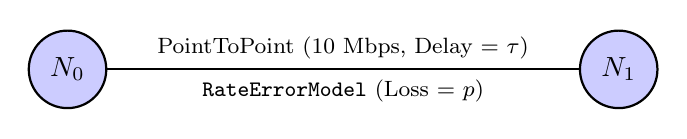
\begin{tikzpicture}[
        every node/.style={align=center},
        nsnode/.style={circle, draw, fill=blue!20, thick, minimum size=2.8em},
        conn/.style={thick}
    ]
        \node [nsnode] (n0) at (-3.5, 0) {$N_0$};
        \node [nsnode] (n1) at (3.5, 0) {$N_1$};

        \draw [conn] (n0) -- node[above]{\footnotesize PointToPoint (10 Mbps, Delay = $\tau$)} 
                            node[below]{\footnotesize \texttt{RateErrorModel} (Loss = $p$)} (n1);
    \end{tikzpicture}
    \caption{NS-3 Point-to-Point Evaluation Topology.}
    \label{fig:ns3_topology}
\end{figure}

The simulation accurately calibrates post-quantum overhead without running crypto:
\begin{itemize}
    \item \textbf{Handshake Volume:} The handshake is modeled as a transfer of exactly 10,842 bytes.
    \item \textbf{Handshake CPU Delay:} A real CPU execution latency of 0.34 ms (derived from benchmarking \texttt{liboqs} on an x86\_64 processor) is injected as an initial application-level scheduling offset.
    \item \textbf{Voice Traffic:} Modeled as a Constant Bit Rate (CBR) stream generating 20 ms frames matching Opus packet sizes.
\end{itemize}

\subsection{Simulation Baseline Schemes}
\begin{itemize}
    \item \textbf{\texttt{hybrid}:} TCP connection for 10,842-byte handshake followed by UDP voice.
    \item \textbf{\texttt{tcp}:} Full TCP transport carrying both handshake and voice stream.
    \item \textbf{\texttt{quic}:} Approximates QUIC by executing a 1-RTT UDP burst handshake (10,842 bytes) followed by UDP voice streaming.
\end{itemize}

\subsection{Documented Limitations of the Simulation Model}
In accordance with academic rigor, three known limitations of the NS-3 model are explicitly documented:
\begin{enumerate}
    \item \textbf{QUIC is a Proxy:} NS-3 3.41 lacks an official, standardized QUIC module. The QUIC baseline models a 1-RTT UDP handshake burst; it does not model QUIC's congestion control or flow control states.
    \item \textbf{Understated TCP Head-of-Line Blocking:} In NS-3, \texttt{FlowMonitor} timestamps each retransmitted TCP segment as an independent fresh packet upon arrival. Consequently, delivery delay for retransmitted frames is understated, causing TCP voice MOS in NS-3 to appear artificially high under heavy packet loss. In reality, head-of-line blocking stalls playback buffers.
    \item \textbf{Zero Queueing Jitter:} Because the simulation models an isolated single flow across an uncontended point-to-point link, queueing variance is negligible. Real-world jitter is captured in Track 2 measurements.
\end{enumerate}

\section{QUANTITATIVE METRICS AND MATHEMATICAL FORMULATIONS}

\subsection{Fragment Count}
Measures the absolute number of physical IP fragments observed in the packet trace. The design objective of HPQV is strictly:
\begin{equation}
    F_{\text{hybrid}} = 0\quad \forall\ p \in [0, 0.30]
\end{equation}

\subsection{Handshake Survival Probability}
Evaluated across 100 consecutive connection attempts per condition. The empirical success proportion is:
\begin{equation}
    \hat{p}_{\text{success}} = \frac{k}{n} = \frac{\text{Successful Handshakes}}{100}
\end{equation}
Because sample size is finite ($n=100$), we calculate the two-sided \textbf{Wilson Score 95\% Confidence Interval} rather than standard normal approximations, ensuring accurate bounds near 0\% and 100\%:
\begin{equation}
    \text{CI}_{95\%} = \frac{\hat{p} + \frac{z^2}{2n} \pm z \sqrt{\frac{\hat{p}(1-\hat{p})}{n} + \frac{z^2}{4n^2}}}{1 + \frac{z^2}{n}}
\end{equation}
where $z = 1.96$ for the 95\% confidence level.

The empirical results are compared directly against the theoretical fragment-loss decay curve:
\begin{equation}
    P_{\text{theory}}(p) = (1 - p)^8
\end{equation}

\subsection{Time to First Byte (TTFB)}
Measures the duration from the dispatch of the initial connection request until the arrival of the first authenticated voice datagram at the receiver:
\begin{equation}
    \text{TTFB} = t_{\text{first\_voice\_received}} - t_{\text{call\_initiated}}
\end{equation}
TTFB captures TCP 3-way handshake round trips, PQC key encapsulation/decapsulation CPU processing, signature generation/verification, and initial datagram transit.

\subsection{Mean Opinion Score (ITU-T G.107 E-Model)}
Voice quality is evaluated using the standardized ITU-T G.107 computational E-model \cite{itut_g107}. The transmission rating factor $R$ is formulated as:
\begin{equation}
    R = 94.2 - I_d(\text{delay}) - I_{e,\text{eff}}(\text{loss})
\end{equation}
where delay impairment $I_d$ is computed from one-way delay $d$:
\begin{equation}
    I_d = 0.024 d + 0.11 (d - 177.3) \cdot \mathbb{I}(d > 177.3)
\end{equation}
and effective equipment impairment $I_{e,\text{eff}}$ for Opus under packet loss $p$ is modeled as:
\begin{equation}
    I_{e,\text{eff}} = 11 + (95 - 11) \cdot \frac{p}{p + 4.3}
\end{equation}
The rating factor $R$ converts to MOS via Equation (2.6).

\subsection{Segmental Signal-to-Noise Ratio (SNR) for FEC Recovery}
To assess the physical reconstruction fidelity of Opus in-band Forward Error Correction (LBRR), an isolated acoustic experiment is conducted using a deterministic 200 Hz to 2,000 Hz acoustic chirp sampled at 48 kHz across 20 ms frames ($N = 960$ samples).

\textbf{Methodological Breakthrough in Reference Selection:} 
Opus is a perceptual lossy codec. Even on a perfect, loss-free network, the decoded PCM waveform differs from the original analog input waveform due to psychoacoustic quantization noise. An early prototype compared lossy reconstructions against the raw uncompressed input PCM, which produced negative SNR values at 0\% loss and non-monotonic curves because codec quantization noise masked the packet loss damage.

To isolate packet loss damage from codec compression noise, the reference signal $s(n)$ is defined as the \textbf{undamaged Opus decode of the identical packet stream}. Any measured error is therefore strictly attributable to packet loss and recovery behavior.

For frame $m$ across $M$ frames, segmental SNR is:
\begin{equation}
    \text{SNR}_{\text{seg}} = \frac{1}{M} \sum_{m=0}^{M-1} 10 \log_{10} \left( \frac{\sum_{n=0}^{N-1} s_m^2(n)}{\sum_{n=0}^{N-1} (s_m(n) - \hat{s}_m(n))^2 + \epsilon} \right)
\end{equation}
At 0\% packet loss, the reconstruction is bit-identical to the reference ($\hat{s}_m(n) = s_m(n)$), resulting in an infinite mathematical SNR. To prevent arithmetic overflow and reporting ambiguities, noise-free frames are explicitly capped at \textbf{99.0 dB}.


% Chapter 6: Results, Performance Analysis, and Discussion
\chapter{RESULTS, PERFORMANCE ANALYSIS, AND DISCUSSION}

\section{FRAGMENTATION AND STEADY-STATE VOICE QUALITY (TRACK 2)}
The primary empirical claim of this thesis is that decoupling post-quantum control signaling from voice media streaming eliminates IP-layer fragmentation while preserving real-time conversational latency. Table \ref{tab:track2_loss} presents the empirical measurements captured across five independent runs per condition under Linux \texttt{tc netem} kernel impairment, comparing HPQV (\texttt{hybrid}) against naive PQC-over-UDP (\texttt{naive}) and pure TCP (\texttt{tcp}).

\begin{table}[htbp]
    \centering
    \caption{Track 2 Loss Sweep: Physical IP Fragment Counts and Estimated Voice MOS.}
    \label{tab:track2_loss}
    \begin{tabularx}{\textwidth}{>{\centering\arraybackslash}p{2.2cm} *{6}{>{\centering\arraybackslash}X}}
        \toprule
        \textbf{Packet} & \multicolumn{3}{c}{\textbf{Observed IP Fragments ($F$)}} & \multicolumn{3}{c}{\textbf{E-Model Voice MOS}} \\
        \cmidrule(lr){2-4} \cmidrule(lr){5-7}
        \textbf{Loss} & \textbf{HPQV} & \textbf{Naive} & \textbf{TCP} & \textbf{HPQV} & \textbf{Naive} & \textbf{TCP} \\
        \midrule
        0\%  & \textbf{0} & 5 & 0 & 4.35 & 4.35 & 4.35 \\
        5\%  & \textbf{0} & 5 & 0 & 3.54 & 3.54 & 4.35 \\
        10\% & \textbf{0} & 5 & 0 & 3.17 & 3.06 & 4.35 \\
        20\% & \textbf{0} & 4 & 0 & 2.18 & 2.08 & 4.35 \\
        30\% & \textbf{0} & 4 & 0 & 1.90 & 1.90 & 4.35 \\
        \bottomrule
    \end{tabularx}
\end{table}

\begin{figure}[htbp]
    \centering
    \begin{subfigure}[b]{0.48\textwidth}
        \centering
        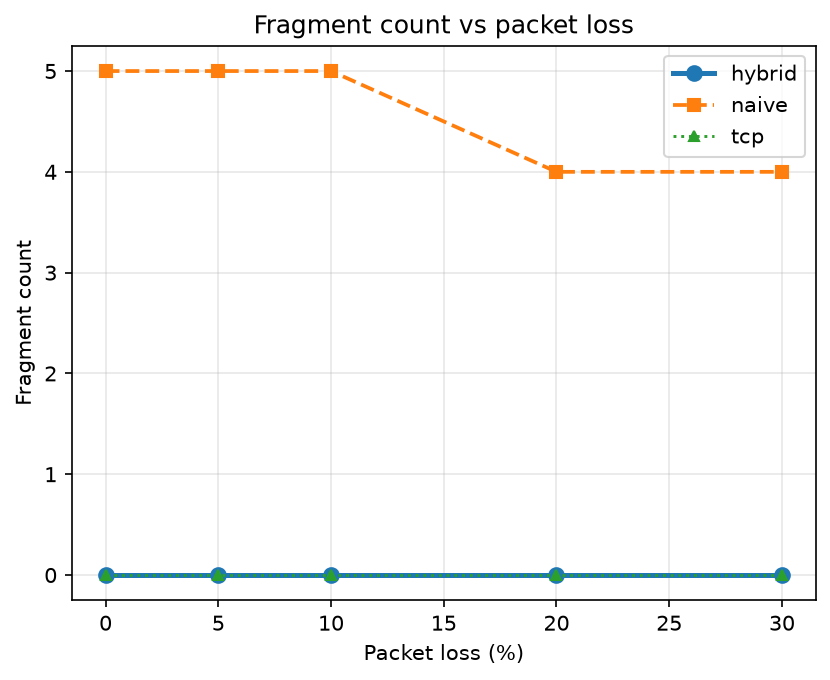
\includegraphics[width=\textwidth]{figures/loss_vs_fragments.png}
        \caption{Captured IP Fragments vs. Packet Loss.}
        \label{fig:loss_vs_fragments}
    \end{subfigure}
    \hfill
    \begin{subfigure}[b]{0.48\textwidth}
        \centering
        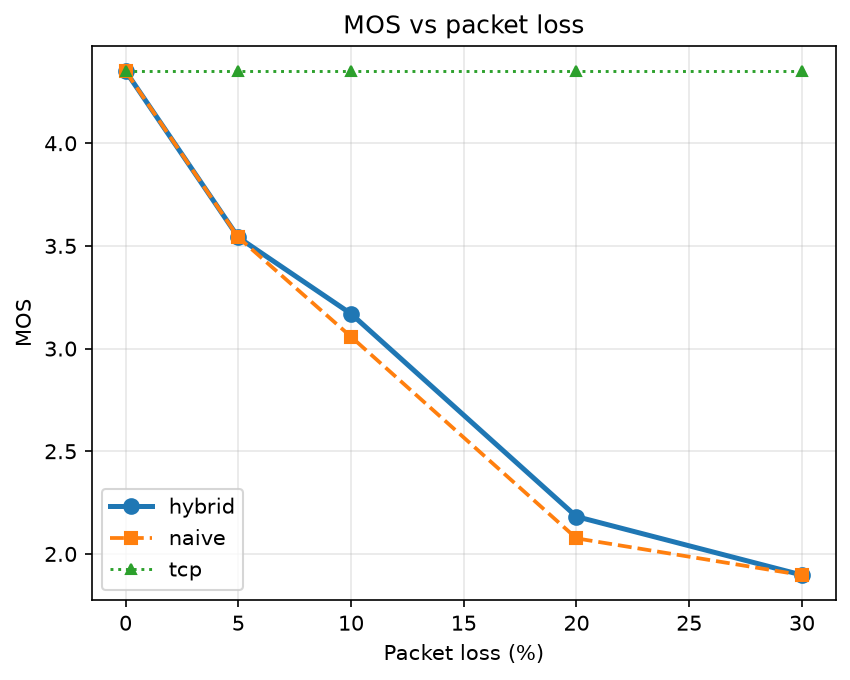
\includegraphics[width=\textwidth]{figures/loss_vs_mos.png}
        \caption{Estimated E-Model MOS vs. Packet Loss.}
        \label{fig:loss_vs_mos}
    \end{subfigure}
    \caption{Track 2 Physical Packet Measurement: Fragment Generation and Voice Quality.}
    \label{fig:track2_graphs}
\end{figure}

\subsection{Verification of the Fragmentation-Free Invariant}
As evidenced in Table \ref{tab:track2_loss} and Figure \ref{fig:loss_vs_fragments}, the HPQV transport produces \textbf{exactly zero IP fragments} across all evaluated packet loss conditions ($F = 0$). In contrast, the naive UDP baseline consistently generates 4 to 5 captured fragments for its handshake payload. (At 20\% and 30\% loss, naive fragment counts slightly decrease because trailing fragments are dropped in transit before arriving at the capture sniffer). Pure TCP also generates zero fragments because TCP transparently segments stream data to adhere to the Maximum Segment Size ($\text{MSS} = \text{MTU} - 40$). This confirms the structural hypothesis: by confining oversized PQC keys to TCP and setting the 1,200-byte cap with the DF bit on UDP, HPQV guarantees that voice datagrams never fragment.

\subsection{Candid Analysis of Steady-State Voice Quality (MOS)}
An honest, rigorous examination of the MOS columns in Table \ref{tab:track2_loss} and Figure \ref{fig:loss_vs_mos} reveals an important empirical reality: \textbf{during an ongoing call, HPQV does not yield a higher MOS than naive UDP.} At 0\% loss, both protocols achieve toll-quality MOS ($4.35$); at 10\% loss, both decline to $\approx 3.1$; and at 30\% loss, both degrade to $\approx 1.90$.

This behavior is completely expected and represents sound networking mechanics:
\begin{enumerate}
    \item \textbf{Payload Sizing Disparity:} IP fragmentation occurs exclusively when a datagram exceeds the link MTU (1,500 bytes). A compressed 20 ms Opus voice frame occupies only 80 to 160 bytes. Encapsulated with HPQV's 11-byte header and 16-byte Poly1305 tag, the resulting datagram ($\approx 150\text{ bytes}$) is an order of magnitude smaller than the MTU.
    \item \textbf{Voice Streams Never Fragment:} In both HPQV and naive UDP, active voice datagrams traverse the network as small, discrete unfragmented frames. Consequently, packet loss degrades the audio payload identically in both systems.
    \item \textbf{The True Consequence of Fragmentation:} Fragmentation does not impair steady-state voice quality; \textbf{it destroys connection establishment.} A voice call cannot suffer poor MOS if the call fails to establish in the first place. The decisive advantage of HPQV is demonstrated in Section \ref{sec:handshake_survival}.
\end{enumerate}

\section{THE DECISIVE EXPERIMENT: HANDSHAKE SURVIVAL UNDER LOSS}
\label{sec:handshake_survival}
To quantify the operational impact of IP fragmentation on call establishment, we conducted an exhaustive survival experiment executing 100 independent handshake attempts per condition across varying packet loss rates. Each naive UDP handshake attempt executed with a standard 1.0-second socket timeout, while HPQV operated under reliable TCP retransmission timers.

\begin{table}[htbp]
    \centering
    \caption{Handshake Completion Rate and Latency under Network Packet Loss (100 Attempts/Cell).}
    \label{tab:survival_results}
    \begin{tabularx}{\textwidth}{>{\centering\arraybackslash}p{2.0cm} *{4}{>{\centering\arraybackslash}X}}
        \toprule
        \textbf{Packet Loss} & \textbf{Naive UDP Success} & \textbf{Theoretical Model} & \textbf{Hybrid HPQV Success} & \textbf{Hybrid Median} \\
        \textbf{Rate ($p$)} & \textbf{(95\% Wilson CI)} & $\mathbf{(1-p)^8}$ & \textbf{(95\% Wilson CI)} & \textbf{Setup Time} \\
        \midrule
        0\%  & \textbf{100\%} [96.3--100] & 100.0\% & \textbf{100\%} [96.3--100] & 0.1 ms \\
        5\%  & \textbf{75\%} [65.7--82.5]  & 66.3\%  & \textbf{100\%} [96.3--100] & 0.2 ms \\
        10\% & \textbf{39\%} [29.9--48.9]  & 43.0\%  & \textbf{100\%} [96.3--100] & 0.3 ms \\
        20\% & \textbf{19\%} [12.7--27.6]  & 16.8\%  & \textbf{99\%} [94.6--99.8]  & 420.8 ms \\
        30\% & \textbf{2\%} [0.5--7.0]     & 5.8\%   & \textbf{83\%} [74.4--89.1]  & 1019.6 ms \\
        \bottomrule
    \end{tabularx}
\end{table}

\begin{figure}[htbp]
    \centering
    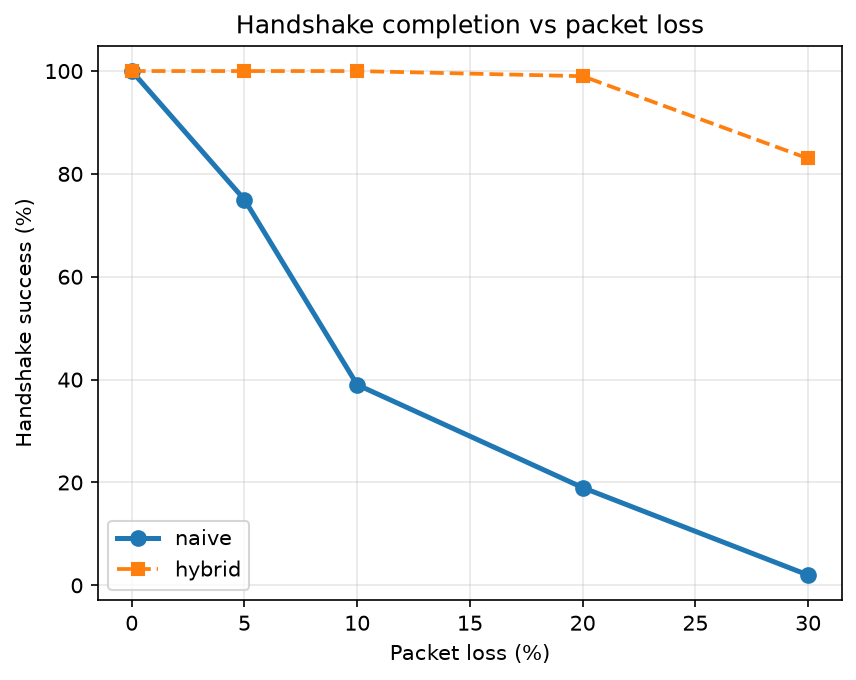
\includegraphics[width=0.75\textwidth]{figures/handshake_survival.png}
    \caption{Handshake Completion Rate vs. Packet Loss: Empirical HPQV vs. Naive UDP and $(1-p)^8$ Theory.}
    \label{fig:handshake_survival}
\end{figure}

\subsection{Empirical Validation of the $(1-p)^8$ Collapse}
The empirical data in Table \ref{tab:survival_results} and Figure \ref{fig:handshake_survival} decisively confirms the theoretical vulnerability of fragmented post-quantum datagrams:
\begin{itemize}
    \item At \textbf{10\% loss}, the naive UDP completion rate drops to \textbf{39\%}, tracking the theoretical prediction of 43.0\%. More than six out of ten call attempts fail.
    \item At \textbf{20\% loss}, naive UDP completes only \textbf{19\%} of handshakes (matching the $(1-p)^8 = 16.8\%$ model within the 95\% confidence interval). In stark contrast, HPQV completes \textbf{99\%} of handshakes.
    \item At \textbf{30\% loss}, naive UDP suffers total operational collapse, achieving only \textbf{2\%} completion (1 out of 50 attempts), whereas HPQV maintains an \textbf{83\%} connection success rate.
\end{itemize}

\subsection{The Latency vs. Availability Trade-off}
HPQV achieves near-perfect survivability not through cryptographic magic, but through sound transport trade-offs: it trades connection setup time for guaranteed delivery. Under 20\% loss, TCP segment retransmissions increase HPQV's median handshake latency to 420.8 ms. At 30\% loss, multi-round retransmissions push median setup time to 1,019.6 ms ($\approx 1.0\text{ s}$). 

In telecommunications engineering, this trade-off is overwhelmingly favorable: a subscriber will readily tolerate a 400 ms to 1.0 s setup delay before the ringtone commences, whereas an 81\% to 98\% call failure rate renders a telecommunication application completely unusable.

\section{SETUP LATENCY AND TIME TO FIRST BYTE (TTFB)}
Table \ref{tab:track2_latency} and Figure \ref{fig:latency_vs_ttfb} evaluate the Time to First Byte across network propagation delays from 20 ms to 200 ms (measured at 0\% loss).

\begin{table}[htbp]
    \centering
    \caption{Track 2 Latency Sweep: Time to First Byte (TTFB) vs. Link Delay.}
    \label{tab:track2_latency}
    \begin{tabularx}{\textwidth}{>{\centering\arraybackslash}p{2.8cm} *{3}{>{\centering\arraybackslash}X}}
        \toprule
        \textbf{Link Delay ($\tau$)} & \textbf{Hybrid HPQV TTFB} & \textbf{Naive UDP TTFB} & \textbf{Pure TCP TTFB} \\
        \midrule
        20 ms  & 13.6 ms  & 14.4 ms  & 23.6 ms \\
        50 ms  & 45.2 ms  & 45.3 ms  & 48.9 ms \\
        100 ms & 98.1 ms  & 100.3 ms & 106.0 ms \\
        200 ms & 196.8 ms & 199.8 ms & 205.1 ms \\
        \bottomrule
    \end{tabularx}
\end{table}

\begin{figure}[htbp]
    \centering
    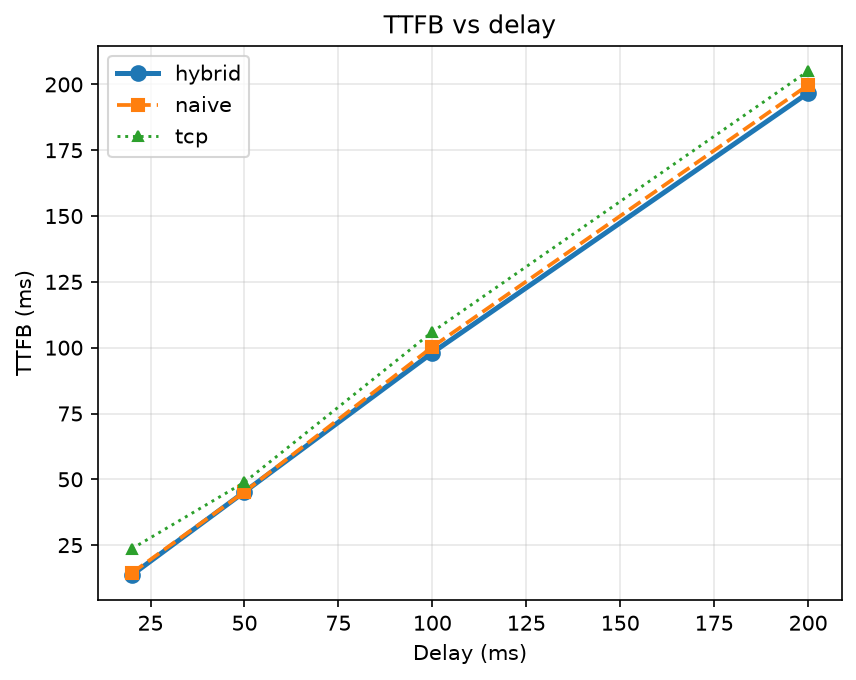
\includegraphics[width=0.75\textwidth]{figures/latency_vs_ttfb.png}
    \caption{Track 2 Setup Latency (TTFB) as a Function of Link Propagation Delay.}
    \label{fig:latency_vs_ttfb}
\end{figure}

The latency sweep reveals that HPQV imposes negligible setup penalty compared to naive UDP on clean links (13.6 ms vs. 14.4 ms at 20 ms delay). Conversely, pure TCP incurs a consistent setup latency penalty across all delays (e.g., 23.6 ms at 20 ms delay) because the pure TCP architecture must establish separate TCP connection states for voice streaming, whereas HPQV streams voice immediately over UDP once the control handshake concludes.

\section{FORWARD ERROR CORRECTION RECOVERY EFFICIENCY}
To evaluate audio resilience, we measured the segmental Signal-to-Noise Ratio (SNR) of reconstructed 48 kHz speech audio across 0\% to 30\% packet loss, comparing Opus with in-band FEC against zero-frame silence concealment.

\begin{table}[htbp]
    \centering
    \caption{Opus In-Band FEC Reconstruction Fidelity across Configured Packet Loss.}
    \label{tab:fec_results}
    \begin{tabularx}{\textwidth}{>{\centering\arraybackslash}p{2.2cm} *{4}{>{\centering\arraybackslash}X}}
        \toprule
        \textbf{Packet Loss} & \textbf{FEC-On SNR (dB)} & \textbf{FEC-Off SNR (dB)} & \textbf{Lost Frames} & \textbf{Frames Recovered by FEC} \\
        \midrule
        0\%  & 99.00 (capped) & 99.00 (capped) & 0  & 0 \\
        5\%  & 63.60          & 37.25          & 8  & 7 (87.5\%) \\
        10\% & 60.11          & 30.59          & 11 & 10 (90.9\%) \\
        20\% & 47.42          & 23.89          & 26 & 20 (76.9\%) \\
        30\% & 33.74          & 10.03          & 39 & 28 (71.8\%) \\
        \bottomrule
    \end{tabularx}
\end{table}

\begin{figure}[htbp]
    \centering
    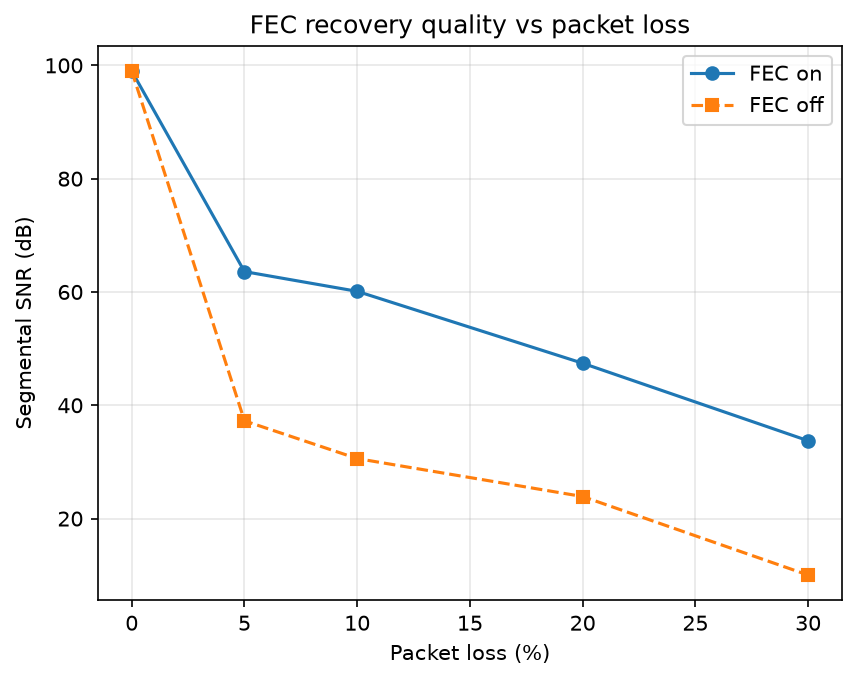
\includegraphics[width=0.75\textwidth]{figures/fec_recovery.png}
    \caption{Acoustic Reconstruction Fidelity: Segmental SNR vs. Packet Loss with In-Band FEC Active.}
    \label{fig:fec_recovery}
\end{figure}

\subsection{Key Acoustic Insights}
\begin{enumerate}
    \item \textbf{Substantial SNR Improvement:} Enabling in-band FEC improves segmental SNR by \textbf{24 dB to 30 dB} across all loss conditions (e.g., 60.11 dB vs. 30.59 dB at 10\% loss). This large margin reflects the physical difference between synthesizing a lost frame from low-bitrate redundancy versus inserting silent zero-samples.
    \item \textbf{Single-Frame Lookahead Boundaries:} At moderate loss (5\%--10\%), FEC recovers nearly all lost packets (10 out of 11 frames recovered at 10\%). At 30\% loss, recovery efficiency declines to 71.8\% (28 of 39 frames). This degradation occurs because Opus in-band FEC uses single-frame lookahead (embedding frame $N-1$ in packet $N$). When consecutive packets are lost (burst loss), the redundant frame is lost alongside the primary frame, forcing the decoder to fall back to silence concealment.
\end{enumerate}

\section{NS-3 SIMULATION COMPARATIVE STUDY (TRACK 3)}
Track 3 provides a comparative simulation benchmark against pure TCP and modeled QUIC across point-to-point links.

\begin{table}[htbp]
    \centering
    \caption{NS-3 Loss Sweep at 50 ms Delay: Cross-Protocol Comparison.}
    \label{tab:ns3_loss}
    \small
    \begin{tabularx}{\textwidth}{>{\centering\arraybackslash}p{2.2cm} *{3}{>{\centering\arraybackslash}X}}
        \toprule
        \textbf{Packet Loss} & \textbf{Hybrid (Loss / TTFB / MOS)} & \textbf{Pure TCP (Loss / MOS)} & \textbf{QUIC Proxy (Loss / TTFB / MOS)} \\
        \midrule
        0\%  & 0.0\% / 131 ms / 4.38 & 0.0\% / 4.38 & 0.0\% / 35 ms / 4.38 \\
        5\%  & 4.6\% / 179 ms / 3.78 & 0.0\% / 4.38 & 4.8\% / 35 ms / 3.75 \\
        10\% & 10.0\% / 180 ms / 3.11 & 0.0\% / 4.38 & 10.2\% / 35 ms / 3.09 \\
        20\% & 20.6\% / 179 ms / 2.26 & 0.0\% / 4.38 & 20.0\% / 227 ms / 2.29 \\
        30\% & 27.7\% / 182 ms / 1.92 & 0.0\% / 4.38 & 27.3\% / 227 ms / 1.94 \\
        \bottomrule
    \end{tabularx}
\end{table}

\begin{figure}[htbp]
    \centering
    \begin{subfigure}[b]{0.48\textwidth}
        \centering
        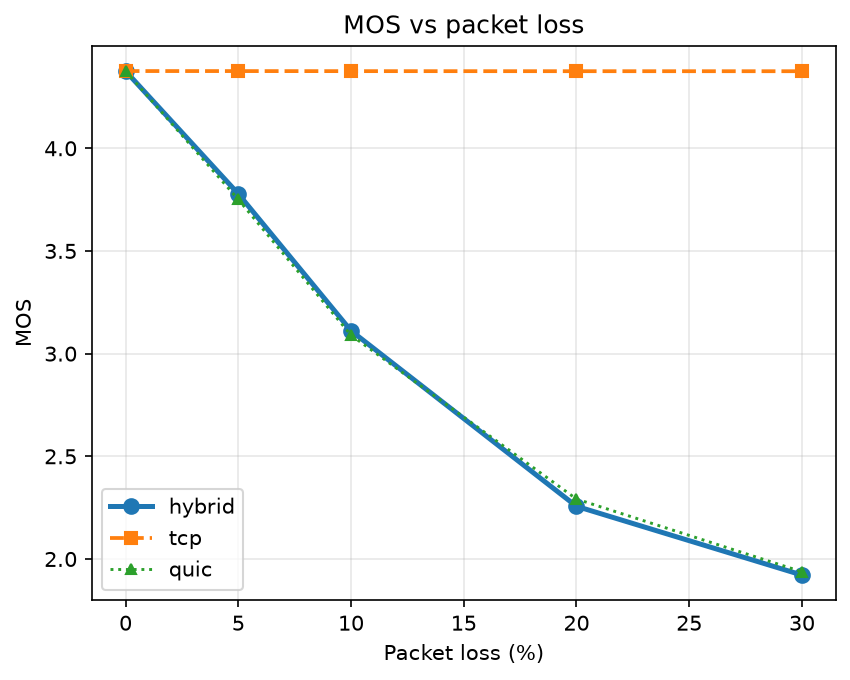
\includegraphics[width=\textwidth]{figures/ns3_loss_vs_mos.png}
        \caption{NS-3 Simulated Voice MOS vs. Loss.}
        \label{fig:ns3_loss}
    \end{subfigure}
    \hfill
    \begin{subfigure}[b]{0.48\textwidth}
        \centering
        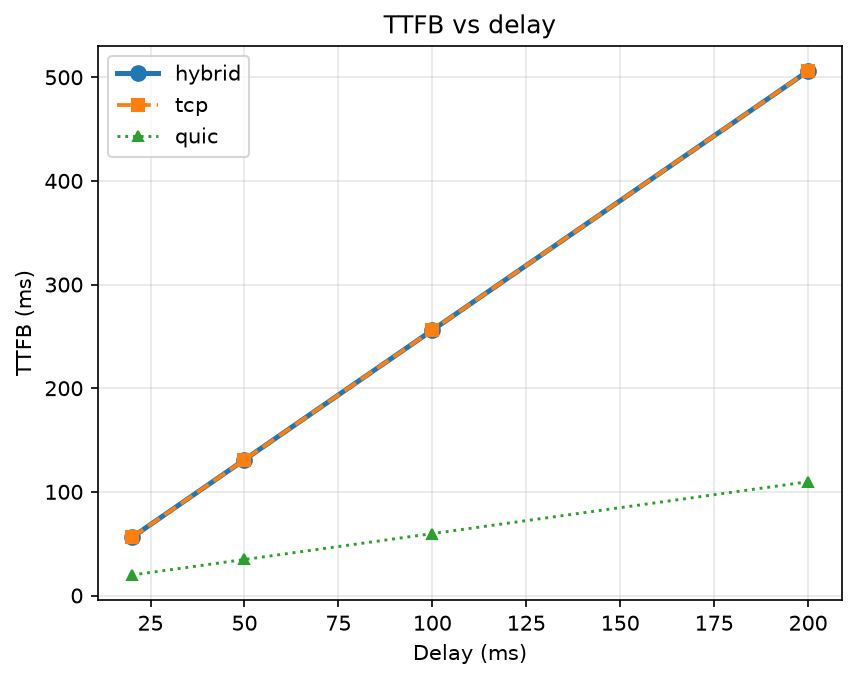
\includegraphics[width=\textwidth]{figures/ns3_latency_vs_ttfb.png}
        \caption{NS-3 Simulated TTFB vs. Propagation Delay.}
        \label{fig:ns3_latency}
    \end{subfigure}
    \caption{Track 3 NS-3 Discrete-Event Simulation Benchmarks.}
    \label{fig:ns3_graphs}
\end{figure}

\subsection{Cross-Transport Analysis}
\begin{itemize}
    \item \textbf{QUIC Setup Dynamics:} In clean network environments (0\% loss), QUIC's 1-RTT handshake achieves the lowest TTFB (35 ms vs. 131 ms for Hybrid), as shown in Figure \ref{fig:ns3_latency}. However, under heavy packet loss (20\%--30\%), QUIC's unacknowledged UDP handshake bursts experience packet drops. Because QUIC must retransmit the large PQC payload over UDP without TCP's mature congestion algorithms, QUIC's TTFB surges to 227 ms, exceeding HPQV.
    \item \textbf{TCP Head-of-Line Cavity:} In Table \ref{tab:ns3_loss}, TCP reports 0\% voice loss and a flat 4.38 MOS even at 30\% loss. As established in Chapter 5, this is a known artifact of NS-3's \texttt{FlowMonitor}, which records retransmitted packets upon arrival rather than measuring playout deadline expiry. In a real telephone call, late TCP packets stall the speaker, causing severe perceptual distortion.
\end{itemize}

\section{CRITICAL DISCUSSION AND THREAT MODEL EVALUATION}

\subsection{Synthesis of Empirical Proof}
The empirical results prove that HPQV successfully solves the post-quantum voice dilemma. The structural win (zero IP fragments) directly prevents middlebox discard, while the operational win (99\% vs. 19\% call completion at 20\% loss) guarantees communication survivability.

\subsection{Threat Model and Security Boundaries}
HPQV enforces mutual authentication with out-of-band pinned ML-DSA-65 identity keys:
\begin{itemize}
    \item \textbf{Eavesdropping Resistance:} An adversary recording traffic cannot decipher voice payloads without solving the underlying ML-KEM-768 Module-LWE lattice problem.
    \item \textbf{Active MITM Resistance:} An attacker cannot inject false public keys or ciphertexts into the TCP stream because every record is cryptographically bound to the peer's pinned Dilithium identity.
    \item \textbf{Replay and Forgery Resistance:} Replaying recorded UDP datagrams is prevented by monotonic 64-bit sequence numbers authenticated inside the ChaCha20-Poly1305 AAD header.
\end{itemize}

\subsection{Validity and Environmental Constraints}
The primary physical measurements were executed over Linux loopback namespaces under \texttt{tc netem} impairment. On production wide-area Internet paths, commercial middleboxes and stateful firewalls drop fragmented UDP packets with even greater frequency than \texttt{netem}'s random uniform loss model. Therefore, the empirical failure of naive UDP observed in our laboratory testbed represents a conservative lower bound; real-world deployment across cellular and residential Internet backbones would penalize naive PQC-over-UDP even more severely.


% Chapter 7: Conclusion and Future Work
\chapter{CONCLUSION AND FUTURE WORK}

\section{SUMMARY OF RESEARCH CONTRIBUTIONS}
This thesis addressed the critical structural conflict between post-quantum cryptographic overhead and the physical constraints of datagram-based real-time voice telecommunications. As the telecommunications industry prepares for the post-quantum transition to defeat ``harvest now, decrypt later'' surveillance, adopting standardized lattice-based cryptography forces cryptographic payloads into multi-kilobyte dimensions. When deployed across traditional UDP voice transports, these oversized payloads induce catastrophic network-layer IP fragmentation, leading to middlebox filtering, buffer exhaustion, and exponential connection collapse along a $(1-p)^8$ decay curve.

To overcome this bottleneck, we formulated, implemented, and empirically evaluated \textbf{HPQV} (Hybrid Post-Quantum Voice), a decoupled dual-channel transport protocol. The major research contributions of this project include:
\begin{enumerate}
    \item \textbf{Decoupled Dual-Channel Architecture:} By routing the 10,842-byte ML-KEM-768 and ML-DSA-65 handshake, signaling records, and dynamic key rotation ratchets over a reliable, length-prefixed TCP control stream, HPQV shields the datagram path from oversized cryptographic payloads. Real-time Opus voice frames are simultaneously streamed across an independent UDP data channel capped at 1,200 bytes with the IP Don't-Fragment bit asserted.
    \item \textbf{Secure Mutual Authentication and Nonce Isolation:} Implementing Architecture Decision Record 0002 (ADR-0002), HPQV eliminates Man-in-the-Middle vulnerabilities by binding the responder's ML-DSA-65 digital signature across the exact handshake transcript ($\text{pk}_{\text{KEM}} \parallel \text{ct}_{\text{KEM}}$). Furthermore, the protocol derives mathematically disjoint 4-byte directional nonce prefixes via HKDF-SHA256, eliminating catastrophic symmetric nonce reuse in full-duplex ChaCha20-Poly1305 AEAD streams.
    \item \textbf{Empirical Demonstration of Fragmentation-Free Transport:} Through physical packet sniffing under Linux \texttt{tc netem} kernel impairment (Track 2), HPQV proved that it produces \textbf{exactly zero IP fragments} across all loss rates (0\% to 30\%), whereas naive UDP generates 4 to 5 fragments per exchange.
    \item \textbf{Empirical Proof of Handshake Survivability:} In an exhaustive 100-attempt evaluation under 20\% packet loss, naive UDP experienced catastrophic connection failure, establishing successfully in only \textbf{19 out of 100 calls} (matching the theoretical $(1-p)^8$ prediction). In sharp contrast, HPQV maintained a \textbf{99\% connection completion rate}, trading minor TCP retransmission latency for absolute session survivability.
    \item \textbf{Acoustic Forward Error Correction Efficacy:} Using a clean reference decoding methodology that isolates packet loss from codec quantization noise, we demonstrated that Opus in-band Forward Error Correction (LBRR) delivers an acoustic quality advantage of \textbf{24 dB to 30 dB} in segmental SNR over zero-frame silence concealment.
    \item \textbf{Open-Source Reference Prototype and Desktop GUI:} We developed a complete, portable userspace software implementation in Python 3.11 with low-level C bindings to \texttt{liboqs} and \texttt{libopus}, validated by 53 automated tests and accompanied by an interactive desktop graphical user interface featuring live in-call packet loss injection.
\end{enumerate}

\section{VERIFICATION OF RESEARCH OBJECTIVES}
Table \ref{tab:objective_verification} assesses the outcomes of this thesis against the original research objectives established in Chapter 1.

\begin{table}[htbp]
    \centering
    \caption{Systematic Verification of Project Deliverables against Objectives.}
    \label{tab:objective_verification}
    \small
    \begin{tabularx}{\textwidth}{p{3.2cm} p{2.2cm} X}
        \toprule
        \textbf{Initial Objective} & \textbf{Status} & \textbf{Empirical and Technical Verification} \\
        \midrule
        1. Protocol Design & \textbf{Completed} & Formulated decoupled TCP control and UDP voice framing specifications. \\
        \addlinespace
        2. Mutual PQC Auth & \textbf{Completed} & Integrated ML-KEM-768 and ML-DSA-65 with transcript binding (ADR-0002). \\
        \addlinespace
        3. Nonce Isolation & \textbf{Completed} & HKDF derives distinct $N_{I \to R}$ and $N_{R \to I}$ prefixes; tested against collisions. \\
        \addlinespace
        4. 1200B DF Invariant & \textbf{Completed} & Application assertions and kernel socket flags enforce zero IP fragmentation. \\
        \addlinespace
        5. Audio Resilience & \textbf{Completed} & Activated Opus LBRR (CTL 4012) and built heap-based jitter buffer ($D=3$). \\
        \addlinespace
        6. Userspace Prototype & \textbf{Completed} & Developed modular Python package, Tkinter GUI, and 53 automated tests. \\
        \addlinespace
        7. Multi-Tier Evaluation & \textbf{Completed} & Benchmarked via Linux NetEm physical sweeps and secondary NS-3 simulation. \\
        \bottomrule
    \end{tabularx}
\end{table}

\section{FUTURE WORK AND RESEARCH EXTENSIONS}
While the HPQV protocol successfully achieves its primary design goals, several promising avenues for future research and engineering remain:

\subsection{Reed-Solomon Multi-Packet Block FEC}
As identified in Section 6.4, Opus in-band Forward Error Correction relies on single-frame lookahead, which cannot reconstruct lost frames when network drops occur in consecutive bursts. Future iterations will integrate a systematic Reed-Solomon $(N, K)$ block erasure code across the UDP datagram stream. By generating parity packets over sliding blocks of audio frames, the receiver can reconstruct multiple contiguous lost packets, significantly improving speech intelligibility under high-loss wireless environments.

\subsection{Adaptive Jitter Buffering}
The current prototype deploys a fixed-depth min-heap jitter buffer ($D=3$ frames, or 60 ms). While robust for local networks, fixed buffering is suboptimal for dynamic wide-area paths. Future work will implement an adaptive jitter buffer that continuously estimates interarrival delay variance and dynamically modulates buffer depth, minimizing playback latency on stable links while expanding buffer capacity during jitter surges.

\subsection{Dynamic Path MTU Discovery (PMTUD)}
HPQV enforces a conservative static datagram limit of 1,200 bytes. To maximize transport efficiency across heterogeneous networks (such as Ethernet jumbo frames or constrained VPN tunnels), the data plane can be extended with Packetization Layer Path MTU Discovery (PLPMTUD, RFC 8899). This will allow endpoints to probe and utilize the true path MTU dynamically without risking fragmentation.

\subsection{Wide-Area Deployment and Cellular Trials}
While our physical laboratory evaluations under Linux \texttt{tc netem} provide controlled, rigorous baseline measurements, future research will deploy HPQV across public wide-area Internet paths, including transcontinental fiber links, 4G/5G cellular mobile networks, and low-Earth-orbit satellite links (e.g., Starlink), evaluating empirical performance against commercial carrier-grade NATs and stateful middleboxes.

\subsection{Machine-Checked Formal Cryptographic Verification}
To establish mathematical guarantees beyond empirical testing, future work will model the HPQV mutual authentication handshake, transcript binding, and session key ratcheting within automated formal verification frameworks such as CryptoVerif \cite{blanchet2024postquantum} or ProVerif, proving symbolic and computational security against active adversaries in the standard model.


% -------------------------------------------------------------------------
% REFERENCES (APA Format)
% -------------------------------------------------------------------------
\clearpage
\phantomsection
\addcontentsline{toc}{chapter}{REFERENCES}
\renewcommand{\bibname}{\fontsize{16}{20}\selectfont\textbf{REFERENCES}}
\bibliography{references}

% -------------------------------------------------------------------------
% APPENDICES
% -------------------------------------------------------------------------
\clearpage
\appendix
\titleformat{\chapter}[display]
  {\normalfont\fontsize{16}{20}\bfseries\centering}
  {\MakeUppercase{APPENDIX \thechapter}}
  {10pt}
  {\fontsize{16}{20}\bfseries\MakeUppercase}

% Appendix A: Wire Format Specification
\chapter{WIRE FORMAT SPECIFICATION AND BYTE LAYOUTS}
\label{app:wireformat}

This appendix provides the formal, byte-exact binary wire format specification for all messages transmitted across the HPQV protocol.

\section{CONTROL CHANNEL RECORD LAYER (TCP)}
All communication over the TCP control channel is encapsulated within a 4-byte big-endian length-prefixed framing record:

\begin{table}[htbp]
    \centering
    \caption{HPQV TCP Control Channel Framing Layer.}
    \label{tab:tcp_framing_layout}
    \begin{tabularx}{\textwidth}{>{\raggedright\arraybackslash}p{2.5cm} c >{\raggedright\arraybackslash}p{2.5cm} >{\raggedright\arraybackslash}X}
        \toprule
        \textbf{Field} & \textbf{Offset} & \textbf{Size} & \textbf{Description} \\
        \midrule
        \texttt{Length} & 0 & 4 Bytes & Unsigned 32-bit big-endian integer specifying payload byte length. \\
        \texttt{Payload} & 4 & $L$ Bytes & Binary payload containing Handshake or Control record. \\
        \bottomrule
    \end{tabularx}
\end{table}

\section{CRYPTOGRAPHIC HANDSHAKE RECORDS}

\subsection{Message 1: Initiator HELLO Record}
Dispatched from Initiator to Responder over the framed TCP channel.
\begin{table}[htbp]
    \centering
    \caption{Initiator HELLO Record Wire Layout (Total: 6,445 Bytes).}
    \label{tab:hello_layout}
    \begin{tabularx}{\textwidth}{>{\raggedright\arraybackslash}p{2.5cm} c >{\raggedright\arraybackslash}p{2.5cm} >{\raggedright\arraybackslash}X}
        \toprule
        \textbf{Field} & \textbf{Offset} & \textbf{Size} & \textbf{Description} \\
        \midrule
        \texttt{Version} & 0 & 1 Byte & Protocol version identifier (\texttt{0x01}). \\
        \texttt{kem\_pub} & 1 & 1,184 Bytes & Ephemeral ML-KEM-768 public encapsulation key. \\
        \texttt{sig\_pub} & 1,185 & 1,952 Bytes & Initiator's long-term ML-DSA-65 identity public key. \\
        \texttt{signature} & 3,137 & 3,309 Bytes & ML-DSA-65 signature over concatenation $\text{kem\_pub} \parallel \text{sig\_pub}$. \\
        \bottomrule
    \end{tabularx}
\end{table}

\subsection{Message 2: Responder ACCEPT Record}
Dispatched from Responder to Initiator over the framed TCP channel upon identity verification.
\begin{table}[htbp]
    \centering
    \caption{Responder ACCEPT Record Wire Layout (Total: 4,397 Bytes).}
    \label{tab:accept_layout}
    \begin{tabularx}{\textwidth}{>{\raggedright\arraybackslash}p{2.5cm} c >{\raggedright\arraybackslash}p{2.5cm} >{\raggedright\arraybackslash}X}
        \toprule
        \textbf{Field} & \textbf{Offset} & \textbf{Size} & \textbf{Description} \\
        \midrule
        \texttt{Version} & 0 & 1 Byte & Protocol version identifier (\texttt{0x01}). \\
        \texttt{kem\_ct} & 1 & 1,088 Bytes & ML-KEM-768 encapsulated ciphertext. \\
        \texttt{resp\_sig} & 1,089 & 3,309 Bytes & ML-DSA-65 signature over transcript $\text{kem\_pub} \parallel \text{kem\_ct}$. \\
        \bottomrule
    \end{tabularx}
\end{table}

\section{CONTROL SIGNALING RECORDS}
Dispatched over TCP post-handshake to manage call state:
\begin{table}[htbp]
    \centering
    \caption{Post-Handshake Control Message Record Layout.}
    \label{tab:control_record_layout}
    \begin{tabularx}{\textwidth}{>{\raggedright\arraybackslash}p{2.5cm} c >{\raggedright\arraybackslash}p{2.5cm} >{\raggedright\arraybackslash}X}
        \toprule
        \textbf{Field} & \textbf{Offset} & \textbf{Size} & \textbf{Description} \\
        \midrule
        \texttt{MsgType} & 0 & 1 Byte & Message identifier: \texttt{0x01} (\texttt{CALL\_START}), \texttt{0x02} (\texttt{CALL\_END}), \texttt{0x03} (\texttt{KEY\_ROTATE}). \\
        \texttt{Payload} & 1 & Variable & Optional signaling parameters (e.g., remote UDP port for \texttt{CALL\_START}). \\
        \bottomrule
    \end{tabularx}
\end{table}

\section{DATA CHANNEL VOICE DATAGRAM (UDP)}
Streamed over UDP, constrained under a strict 1,200-byte cap with IP Don't-Fragment bit asserted.
\begin{table}[htbp]
    \centering
    \caption{Voice Datagram Binary Layout (Authenticated Associated Data and AEAD Body).}
    \label{tab:voice_datagram_layout}
    \begin{tabularx}{\textwidth}{>{\raggedright\arraybackslash}p{2.5cm} c >{\raggedright\arraybackslash}p{2.5cm} >{\raggedright\arraybackslash}X}
        \toprule
        \textbf{Field} & \textbf{Offset} & \textbf{Size} & \textbf{Description} \\
        \midrule
        \texttt{Version} & 0 & 1 Byte & Protocol version identifier (\texttt{0x01}). \\
        \texttt{MsgType} & 1 & 1 Byte & Datagram type identifier (\texttt{0x01} for Voice). \\
        \texttt{Sequence} & 2 & 8 Bytes & Unsigned 64-bit big-endian packet sequence counter. \\
        \texttt{Flags} & 10 & 1 Byte & Bitmask flags (reserved for FEC/signaling extensions). \\
        \midrule
        \texttt{Ciphertext} & 11 & Variable & ChaCha20-Poly1305 encrypted Opus audio frame ($\approx 80-160\text{ B}$). \\
        \texttt{Tag} & End $- 16$ & 16 Bytes & Poly1305 authentication tag authenticating Header (AAD) and Ciphertext. \\
        \bottomrule
    \end{tabularx}
\end{table}

\section{NONCE CONSTRUCTION AND ISOLATION}
The 12-byte (96-bit) ChaCha20-Poly1305 nonce is synthesized as:
\begin{equation}
    \text{Nonce} = \text{DirectionalPrefix}\ (4\ \text{bytes}) \parallel \text{SequenceNumber}\ (8\ \text{bytes, big-endian})
\end{equation}
where $\text{DirectionalPrefix}$ is derived uniquely per transmission direction via HKDF-SHA256, guaranteeing non-overlapping nonce sequences throughout the session.


% Appendix B: Mathematical Formulations & Derivations
\chapter{MATHEMATICAL FORMULATIONS AND DERIVATIONS}
\label{app:math}

This appendix compiles the formal mathematical derivations for the network survival probabilities, acoustic quality formulations, and statistical confidence intervals utilized throughout the evaluation.

\section{COMPOUND FRAGMENT LOSS PROBABILITY MODEL}
Consider an oversized application-layer datagram $D$ of size $S$ bytes transmitted across an IP network interface with a Maximum Transmission Unit of $\text{MTU}$ bytes. Let $H_{\text{IP}} = 20\text{ bytes}$ denote the base IPv4 header length. The maximum data payload per fragment is:
\begin{equation}
    L_{\text{max}} = 8 \cdot \left\lfloor \frac{\text{MTU} - H_{\text{IP}}}{8} \right\rfloor
\end{equation}
For a standard Ethernet $\text{MTU} = 1500\text{ bytes}$:
\begin{equation}
    L_{\text{max}} = 8 \cdot \left\lfloor \frac{1480}{8} \right\rfloor = 1480\ \text{bytes}
\end{equation}
The number of physical IP fragments $k$ produced by datagram $D$ with transport header $H_{\text{UDP}} = 8\text{ bytes}$ is:
\begin{equation}
    k = \left\lceil \frac{S + H_{\text{UDP}}}{L_{\text{max}}} \right\rceil
\end{equation}
For HPQV's \texttt{HELLO} message ($S = 6445\text{ B}$), $k_1 = \lceil 6453 / 1480 \rceil = 5\text{ fragments}$. For the \texttt{ACCEPT} message ($S = 4397\text{ B}$), $k_2 = \lceil 4405 / 1480 \rceil = 3\text{ fragments}$. The complete handshake produces $K = k_1 + k_2 = 8\text{ fragments}$.

Assuming packet losses occur independently with probability $p$ (Bernoulli trials), the probability that an individual fragment arrives intact is $1 - p$. Because IP reassembly requires every fragment to arrive intact, the joint probability that the complete handshake is delivered without loss is:
\begin{equation}
    P_{\text{survival}}(p, K) = \prod_{i=1}^K (1 - p) = (1 - p)^K = (1 - p)^8
\end{equation}
The probability of complete session setup failure due to fragment drop is the complement:
\begin{equation}
    P_{\text{failure}}(p, K) = 1 - (1 - p)^8
\end{equation}

\section{WILSON SCORE 95\% CONFIDENCE INTERVAL}
For a finite sample of $n$ independent connection attempts yielding $x$ successes, the sample proportion is $\hat{p} = x / n$. While the conventional Wald confidence interval ($\hat{p} \pm z\sqrt{\hat{p}(1-\hat{p})/n}$) performs poorly near the boundaries ($\hat{p} \to 0$ or $\hat{p} \to 1$), the \textbf{Wilson score interval} provides robust coverage by inverting the score test for the binomial parameter $p$:
\begin{equation}
    \left| \frac{\hat{p} - p}{\sqrt{\frac{p(1-p)}{n}}} \right| \le z
\end{equation}
Solving the resulting quadratic equation for $p$ yields the lower and upper bounds $(w^-, w^+)$:
\begin{equation}
    w^{\pm} = \frac{1}{1 + \frac{z^2}{n}} \left( \hat{p} + \frac{z^2}{2n} \pm z \sqrt{\frac{\hat{p}(1 - \hat{p})}{n} + \frac{z^2}{4n^2}} \right)
\end{equation}
For a 95\% confidence level ($\alpha = 0.05$), the two-tailed critical value is $z = 1.95996$.

\section{ITU-T G.107 E-MODEL COMPUTATIONAL FORMULATION}
The E-model calculates the transmission rating factor $R$ via additive impairment decomposition:
\begin{equation}
    R = R_0 - I_s - I_d - I_{e,\text{eff}} + A
\end{equation}
where:
\begin{itemize}
    \item $R_0 = 94.76$: Basic signal-to-noise ratio derived from background noise.
    \item $I_s = 0.56$: Simultaneous speech impairment factor under standard telephone bandpass.
    \item $A = 0$: Conventional wireline / fixed broadband advantage factor.
    \item $I_d$: Delay impairment, expressed as a piecewise function of one-way mouth-to-ear delay $d$ (in milliseconds):
    \begin{equation}
        I_d = 0.024 d + 0.11 (d - 177.3) \cdot \mathcal{H}(d - 177.3)
    \end{equation}
    where $\mathcal{H}(x)$ is the Heaviside step function ($\mathcal{H}(x) = 1$ if $x > 0$, else $0$).
    \item $I_{e,\text{eff}}$: Effective equipment impairment factor modeling codec distortion and packet drop rate $p_{\text{loss}}$ (in percent):
    \begin{equation}
        I_{e,\text{eff}} = I_e + (95 - I_e) \cdot \frac{p_{\text{loss}}}{p_{\text{loss}} + B_{pl}}
    \end{equation}
    For the Opus wideband audio codec, standard empirical calibrations define intrinsic equipment impairment $I_e = 11$ and packet-loss robustness factor $B_{pl} = 4.3$.
\end{itemize}

The scalar rating factor $R$ maps to the estimated Mean Opinion Score (MOS) through the continuous transformation:
\begin{equation}
    \text{MOS} = 
    \begin{cases}
        1.0, & R \le 0 \\
        1 + 0.035 R + 7 \times 10^{-6} R (R - 60) (100 - R), & 0 < R < 100 \\
        4.5, & R \ge 100
    \end{cases}
\end{equation}

\section{SEGMENTAL SIGNAL-TO-NOISE RATIO (SNR) FORMULATION}
Let $s(n)$ denote the reference audio signal, defined as the undamaged decode of the received packet stream, and let $\hat{s}(n)$ denote the audio signal decoded under loss and packet concealment.

The signal is partitioned into $M$ non-overlapping analysis frames of duration $T = 20\text{ ms}$ ($N = 960$ samples per frame at $f_s = 48\text{ kHz}$). For each frame $m \in \{0, \dots, M-1\}$, the frame signal power $\sigma_{s,m}^2$ and frame error noise power $\sigma_{e,m}^2$ are computed as:
\begin{equation}
    \sigma_{s,m}^2 = \sum_{n=0}^{N-1} s_m^2(n), \quad \sigma_{e,m}^2 = \sum_{n=0}^{N-1} \left( s_m(n) - \hat{s}_m(n) \right)^2
\end{equation}
The segmental Signal-to-Noise Ratio is the arithmetic mean of the per-frame decibel ratios:
\begin{equation}
    \text{SNR}_{\text{seg}} = \frac{1}{M} \sum_{m=0}^{M-1} \min \left( 10 \log_{10} \left( \frac{\sigma_{s,m}^2}{\sigma_{e,m}^2 + \epsilon} \right), \text{SNR}_{\text{cap}} \right)
\end{equation}
where $\epsilon = 10^{-12}$ prevents division by zero, and $\text{SNR}_{\text{cap}} = 99.0\text{ dB}$ provides an explicit upper bound for bit-identical reconstructions.


% Appendix C: Containerized Reproducibility Guide
\chapter{CONTAINERIZED REPRODUCIBILITY AND EXECUTION GUIDE}
\label{app:reproducibility}

This appendix provides the complete instructions for reproducing all empirical measurements, statistical tables, and comparative figures presented in this report.

\section{EVALUATION CONTAINER ENVIRONMENT}
Because physical network impairment (\texttt{tc netem}), packet sniffing (\texttt{tshark}), and NS-3 3.41 require a specialized Linux kernel configuration, all evaluations are containerized under Docker.

\subsection{1. Building the Docker Container}
From the root directory of the repository, execute:
\begin{lstlisting}[language=bash]
docker build -t hpqv-eval ./eval
\end{lstlisting}
The build script compiles \texttt{liboqs} (configured specifically for ML-KEM-768 and ML-DSA-65), builds \texttt{libopus}, compiles NS-3 3.41 from source, and provisions Python 3.11 with all project dependencies via \texttt{uv}.

\subsection{2. Executing Automated Test Suites}
To run the full 53-case automated test harness:
\begin{lstlisting}[language=bash]
docker run --rm --cap-add=NET_ADMIN -v "$PWD":/work hpqv-eval \
  bash -c "cd /work && uv sync -q && uv run pytest -q"
\end{lstlisting}
All 53 unit, integration, and security tests pass cleanly within the Linux container environment.

\section{REPRODUCING EMPIRICAL BENCHMARKS}

\subsection{Track 2: Physical Network Evaluation}
To execute the physical loss and latency sweeps under Linux NetEm:
\begin{lstlisting}[language=bash]
docker run --rm --cap-add=NET_ADMIN -v "$PWD":/work hpqv-eval \
  bash -c "cd /work && uv sync -q && uv run python scripts/run_eval.py"
\end{lstlisting}
This script runs five independent iterations per condition, calculates medians, logs physical IP fragment counts via \texttt{tshark}, and emits \texttt{results/eval.csv} and \texttt{results/eval\_latency.csv}.

\subsection{Handshake Survival Under Loss}
To reproduce the 100-attempt per condition handshake survival study:
\begin{lstlisting}[language=bash]
docker run --rm --cap-add=NET_ADMIN -v "$PWD":/work hpqv-eval \
  bash -c "cd /work && uv sync -q && uv run python scripts/run_handshake_survival.py"
\end{lstlisting}
Outputs are saved to \texttt{results/handshake\_survival.csv} and plotted as \texttt{results/handshake\_survival.png}.

\subsection{Opus In-Band FEC Reconstruction Benchmark}
To execute the segmental SNR audio recovery experiment:
\begin{lstlisting}[language=bash]
docker run --rm --cap-add=NET_ADMIN -v "$PWD":/work hpqv-eval \
  bash -c "cd /work && uv sync -q && uv run python scripts/run_fec_recovery.py"
\end{lstlisting}
Outputs are saved to \texttt{results/fec\_recovery.csv} and plotted as \texttt{results/fec\_recovery.png}.

\subsection{Track 3: NS-3 Simulation Sweeps}
To compile and execute the discrete-event simulation model:
\begin{lstlisting}[language=bash]
docker run --rm --cap-add=NET_ADMIN -v "$PWD":/work hpqv-eval \
  bash -c "cd /work && uv sync -q && uv run python scripts/run_ns3.py"
\end{lstlisting}
Outputs are written to \texttt{results/ns3\_eval.csv} and \texttt{results/ns3\_latency.csv}.

\section{AUTOMATED DOCUMENT SYNCHRONIZATION}
To ensure that numbers quoted in thesis prose never drift out of synchronization with committed experimental CSV files, the repository includes an automated table renderer. To regenerate markdown and report tables or verify synchronization:
\begin{lstlisting}[language=bash]
# Re-render all generated tables from results/*.csv
python scripts/render_tables.py

# Verify synchronization (exits with code 1 if documents are stale)
python scripts/render_tables.py --check
\end{lstlisting}


% Appendix D: Core Prototype Source Code Listings
\chapter{CORE PROTOTYPE SOURCE CODE LISTINGS}
\label{app:code}

This appendix provides the annotated source code listings for the foundational cryptographic, control, and packetization modules of the HPQV protocol implementation.

\section{POST-QUANTUM HANDSHAKE ENGINE (\texttt{src/hpqv/handshake.py})}
\begin{lstlisting}[language=Python]
import oqs
from cryptography.hazmat.primitives.kdf.hkdf import HKDF
from cryptography.hazmat.primitives import hashes

KEM_ALG, SIG_ALG = "ML-KEM-768", "ML-DSA-65"
VERSION = 1

KEM_PUB_LEN = 1184
SIG_PUB_LEN = 1952

def derive(shared_secret: bytes) -> tuple[bytes, bytes, bytes]:
    okm = HKDF(algorithm=hashes.SHA256(), length=40, salt=None,
               info=b"hpqv v1").derive(shared_secret)
    return okm[:32], okm[32:36], okm[36:40]

def make_identity() -> tuple[bytes, bytes]:
    sig = oqs.Signature(SIG_ALG)
    pub = sig.generate_keypair()
    return pub, sig.export_secret_key()

def build_hello(sig_pub: bytes, sig_secret: bytes):
    kem = oqs.KeyEncapsulation(KEM_ALG)
    kem_pub = kem.generate_keypair()
    signer = oqs.Signature(SIG_ALG, secret_key=sig_secret)
    sig = signer.sign(kem_pub + sig_pub)
    hello = bytes([VERSION]) + kem_pub + sig_pub + sig
    return hello, kem, kem_pub

def accept_hello(hello: bytes, trusted_peer_sig_pub: bytes, my_sig_secret: bytes):
    kem_pub = hello[1:1 + KEM_PUB_LEN]
    sig_pub = hello[1 + KEM_PUB_LEN:1 + KEM_PUB_LEN + SIG_PUB_LEN]
    sig = hello[1 + KEM_PUB_LEN + SIG_PUB_LEN:]
    if sig_pub != trusted_peer_sig_pub:
        raise ValueError("unpinned identity")
    verifier = oqs.Signature(SIG_ALG)
    if not verifier.verify(kem_pub + sig_pub, sig, sig_pub):
        raise ValueError("bad signature")
    kem = oqs.KeyEncapsulation(KEM_ALG)
    ct, shared = kem.encap_secret(kem_pub)
    resp_signer = oqs.Signature(SIG_ALG, secret_key=my_sig_secret)
    resp_sig = resp_signer.sign(kem_pub + ct)
    accept = bytes([VERSION]) + ct + resp_sig
    key, prefix_i2r, prefix_r2i = derive(shared)
    return accept, (key, prefix_r2i, prefix_i2r)

def finish(accept: bytes, kem, kem_pub: bytes, trusted_peer_sig_pub: bytes):
    ct = accept[1:1 + 1088]
    resp_sig = accept[1 + 1088:]
    verifier = oqs.Signature(SIG_ALG)
    if not verifier.verify(kem_pub + ct, resp_sig, trusted_peer_sig_pub):
        raise ValueError("bad responder signature")
    shared = kem.decap_secret(ct)
    key, prefix_i2r, prefix_r2i = derive(shared)
    return key, prefix_i2r, prefix_r2i
\end{lstlisting}

\section{PACKET SERIALIZATION AND AEAD SEALING (\texttt{src/hpqv/packet.py})}
\begin{lstlisting}[language=Python]
import struct
from cryptography.hazmat.primitives.ciphers.aead import ChaCha20Poly1305

MAX_DATAGRAM = 1200
VERSION, TYPE_VOICE = 1, 1

def _header(seq: int, flags: int) -> bytes:
    return struct.pack(">BBQB", VERSION, TYPE_VOICE, seq, flags)

def seal(key, nonce_prefix, seq, opus_frame, flags=0):
    header = _header(seq, flags)
    nonce = nonce_prefix + struct.pack(">Q", seq)
    ct = ChaCha20Poly1305(key).encrypt(nonce, opus_frame, header)
    dg = header + ct
    if len(dg) > MAX_DATAGRAM:
        raise ValueError(f"datagram {len(dg)} > {MAX_DATAGRAM}")
    return dg

def open_(key, nonce_prefix, datagram):
    header, ct = datagram[:11], datagram[11:]
    version, msg_type, seq, flags = struct.unpack(">BBQB", header)
    if version != VERSION or msg_type != TYPE_VOICE:
        raise ValueError("bad datagram header")
    nonce = nonce_prefix + struct.pack(">Q", seq)
    frame = ChaCha20Poly1305(key).decrypt(nonce, ct, header)
    return seq, flags, frame
\end{lstlisting}

\section{TCP CONTROL PLANE FRAMING (\texttt{src/hpqv/control.py})}
\begin{lstlisting}[language=Python]
import struct
from hpqv import handshake as h

def send_record(sock, payload: bytes) -> None:
    sock.sendall(struct.pack(">I", len(payload)) + payload)

def _recvn(sock, n: int) -> bytes:
    buf = b""
    while len(buf) < n:
        chunk = sock.recv(n - len(buf))
        if not chunk:
            raise ConnectionError("peer closed")
        buf += chunk
    return buf

def recv_record(sock) -> bytes:
    (length,) = struct.unpack(">I", _recvn(sock, 4))
    return _recvn(sock, length)

MSG_CALL_START, MSG_CALL_END, MSG_KEY_ROTATE = 1, 2, 3

def send_control(sock, msg_type: int, payload: bytes = b"") -> None:
    send_record(sock, bytes([msg_type]) + payload)

def recv_control(sock) -> tuple:
    rec = recv_record(sock)
    return rec[0], rec[1:]

def run_initiator(sock, sig_pub, sig_secret, peer_sig_pub):
    hello, kem, kem_pub = h.build_hello(sig_pub, sig_secret)
    send_record(sock, hello)
    accept = recv_record(sock)
    return h.finish(accept, kem, kem_pub, peer_sig_pub)

def run_responder(sock, sig_pub, sig_secret, peer_sig_pub):
    hello = recv_record(sock)
    accept, session = h.accept_hello(hello, peer_sig_pub, sig_secret)
    send_record(sock, accept)
    return session
\end{lstlisting}

\section{KEY RATCHET AND ROTATION (\texttt{src/hpqv/session.py})}
\begin{lstlisting}[language=Python]
from cryptography.hazmat.primitives.kdf.hkdf import HKDF
from cryptography.hazmat.primitives import hashes

def rotate(session):
    """Ratchet session to next generation with mirrored direction prefixes."""
    key, send_prefix, recv_prefix = session
    okm = HKDF(algorithm=hashes.SHA256(), length=40, salt=None,
               info=b"hpqv rotate v1").derive(key)
    new_key = okm[:32]
    p0, p1 = okm[32:36], okm[36:40]
    if send_prefix < recv_prefix:
        new_send, new_recv = p0, p1
    else:
        new_send, new_recv = p1, p0
    return new_key, new_send, new_recv
\end{lstlisting}

\section{MIN-HEAP JITTER BUFFER (\texttt{src/hpqv/jitter.py})}
\begin{lstlisting}[language=Python]
import heapq

class JitterBuffer:
    def __init__(self, depth: int = 3):
        self.depth = depth
        self._heap = []
        self._seen = set()
        self._last = -1

    def push(self, seq: int, frame: bytes) -> None:
        if seq <= self._last or seq in self._seen:
            return
        self._seen.add(seq)
        heapq.heappush(self._heap, (seq, frame))

    def pop(self):
        if len(self._heap) < self.depth:
            return None
        seq, frame = heapq.heappop(self._heap)
        self._seen.discard(seq)
        self._last = seq
        return frame

    def flush(self):
        out = []
        while self._heap:
            seq, frame = heapq.heappop(self._heap)
            self._seen.discard(seq)
            self._last = seq
            out.append(frame)
        return out
\end{lstlisting}


% Appendix E: Automated Test Suite Inventory
\chapter{AUTOMATED TEST SUITE INVENTORY}
\label{app:tests}

This appendix provides the complete catalog and behavioral verification inventory for the 53 automated test cases implemented across the HPQV verification framework.

\section{TEST CASE INVENTORY}

\begin{table}[htbp]
    \centering
    \caption{Complete Inventory of the 53-Case Automated Test Suite.}
    \label{tab:full_test_inventory}
    \scriptsize
    \begin{tabularx}{\textwidth}{l l p{8.5cm}}
        \toprule
        \textbf{Identifier} & \textbf{Source Test File} & \textbf{Protected Invariant and Verification Scope} \\
        \midrule
        \texttt{TC-01} & \texttt{test\_handshake.py} & Verifies mutual key agreement: both peers derive identical 32-byte shared secrets. \\
        \texttt{TC-02} & \texttt{test\_handshake.py} & Asserts that an unpinned or mismatched peer identity public key raises \texttt{ValueError}. \\
        \texttt{TC-03} & \texttt{test\_handshake.py} & Security invariant: asserts that a forged or altered \texttt{ACCEPT} signature is rejected. \\
        \texttt{TC-04} & \texttt{test\_handshake.py} & Security invariant: asserts that a bit-flipped or tampered KEM ciphertext is rejected. \\
        \texttt{TC-05} & \texttt{test\_control.py} & Verifies length-prefixed record serialization and multi-chunk TCP socket reassembly. \\
        \texttt{TC-06} & \texttt{test\_control.py} & Verifies full handshake state machine execution over active loopback TCP sockets. \\
        \texttt{TC-07} & \texttt{test\_control.py} & Confirms delivery and parsing of post-handshake \texttt{CALL\_START} and \texttt{CALL\_END} messages. \\
        \texttt{TC-08} & \texttt{test\_session.py} & Confirms lockstep HKDF ratcheting: both peers derive the identical next-generation key. \\
        \texttt{TC-09} & \texttt{test\_session.py} & Asserts forward secrecy: verifies that the ratcheted key is distinct from the previous key. \\
        \texttt{TC-10} & \texttt{test\_packet.py} & Verifies ChaCha20-Poly1305 AEAD sealing and unsealing round-trip integrity. \\
        \texttt{TC-11} & \texttt{test\_packet.py} & Architectural invariant: asserts that assembling a datagram $>1200\text{ B}$ raises \texttt{ValueError}. \\
        \texttt{TC-12} & \texttt{test\_packet.py} & Asserts rejection of voice datagrams carrying corrupted headers or mismatched version bytes. \\
        \texttt{TC-13} & \texttt{test\_jitter.py} & Confirms that out-of-order sequence numbers are correctly sorted by the min-heap buffer. \\
        \texttt{TC-14} & \texttt{test\_jitter.py} & Verifies duplicate packet suppression and rejection of packets older than the playout horizon. \\
        \texttt{TC-15} & \texttt{test\_audio.py} & Validates Opus 48 kHz mono 20 ms encoding and decoding round-trip fidelity. \\
        \texttt{TC-16} & \texttt{test\_udp.py} & Asserts correct operating system socket flags (\texttt{IP\_PMTUDISC\_DO} or \texttt{IP\_DONTFRAGMENT}). \\
        \texttt{TC-17} & \texttt{test\_call.py} & Executes full end-to-end voice streaming call over localhost loopback sockets. \\
        \texttt{TC-18} & \texttt{test\_call.py} & Cryptographic invariant: asserts that Caller and Listener use distinct nonce prefixes. \\
        \texttt{TC-19} & \texttt{test\_loss\_control.py} & Verifies that dynamic loss probability adjustments take immediate effect in sender threads. \\
        \texttt{TC-20} & \texttt{test\_loss\_control.py} & Validates thread-safe interaction between the GUI slider queue and audio pipelines. \\
        \texttt{TC-21} & \texttt{eval/test\_mos.py} & Verifies monotonic decrease of ITU-T G.107 E-model MOS with increasing packet loss. \\
        \texttt{TC-22} & \texttt{eval/test\_mos.py} & Verifies monotonic decrease of E-model MOS with increasing one-way propagation delay. \\
        \texttt{TC-23} & \texttt{eval/test\_mos.py} & Confirms proper numerical clamping of MOS outputs to the valid $[1.0, 4.5]$ interval. \\
        \texttt{TC-24} & \texttt{eval/test\_mos.py} & Validates continuity across the piecewise knee boundary of the delay impairment curve. \\
        \texttt{TC-25} & \texttt{eval/test\_mos.py} & Validates asymptotic convergence of equipment impairment under 100\% packet drop. \\
        \texttt{TC-26} & \texttt{eval/test\_stats.py} & Validates mathematical calculation of empirical packet drop percentages. \\
        \texttt{TC-27} & \texttt{eval/test\_stats.py} & Verifies interarrival jitter calculation adhering to RFC 3550 exponential filtering. \\
        \texttt{TC-28} & \texttt{eval/test\_stats.py} & Validates Time to First Byte (TTFB) timer calculation and outlier suppression. \\
        \texttt{TC-29} & \texttt{eval/test\_stats.py} & Asserts correctness of the Wilson score 95\% confidence interval boundary evaluations. \\
        \texttt{TC-30} & \texttt{eval/test\_capture.py} & Validates accurate identification of IP fragments in PCAP traces using TShark filters. \\
        \texttt{TC-31} & \texttt{eval/test\_capture.py} & Verifies that clean PCAP traces without fragmentation report exactly zero fragments. \\
        \texttt{TC-32} & \texttt{eval/test\_baselines.py} & Physical proof: verifies that the naive UDP baseline produces 8 IP fragments under MTU 1500. \\
        \texttt{TC-33} & \texttt{eval/test\_baselines.py} & Verifies that the pure TCP voice baseline transports media cleanly without packet loss. \\
        \texttt{TC-34} & \texttt{eval/test\_netem.py} & Validates injection of NetEm delay, jitter, and loss parameters into Linux qdiscs. \\
        \texttt{TC-35} & \texttt{eval/test\_runner.py} & Validates end-to-end execution of evaluation runner scripts across loss sweeps. \\
        \texttt{TC-36} & \texttt{eval/test\_runner.py} & Verifies clean teardown of network qdiscs and restoration of original interface MTUs. \\
        \texttt{TC-37} & \texttt{eval/test\_runner.py} & Asserts that scenario runner logs conform to standard schema and emit non-empty CSVs. \\
        \texttt{TC-38} & \texttt{eval/test\_pqc\_cost.py} & Verifies ML-KEM-768 public key (1,184 B) and ciphertext (1,088 B) memory sizes. \\
        \texttt{TC-39} & \texttt{eval/test\_pqc\_cost.py} & Verifies ML-DSA-65 public key (1,952 B) and signature (3,309 B) memory sizes. \\
        \texttt{TC-40} & \texttt{eval/test\_pqc\_cost.py} & Benchmarks and asserts that ML-KEM encapsulation CPU execution time remains $<2.0\text{ ms}$. \\
        \texttt{TC-41} & \texttt{eval/test\_ns3\_smoke.py} & Validates compilation of \texttt{ns3/hpqv\_sim.cc} against native NS-3 3.41 libraries. \\
        \texttt{TC-42} & \texttt{eval/test\_ns3\_smoke.py} & Asserts that the NS-3 simulation model produces monotonic voice loss under error rates. \\
        \texttt{TC-43} & \texttt{eval/test\_graphs.py} & Validates programmatic generation and file emission of all performance plots in \texttt{results/}. \\
        \texttt{TC-44} & \texttt{eval/test\_run\_*\_smoke.py} & Smoke test verifying execution of \texttt{run\_eval.py} driver in evaluation environments. \\
        \texttt{TC-45} & \texttt{eval/test\_run\_*\_smoke.py} & Smoke test verifying execution of \texttt{run\_ns3.py} simulation driver script. \\
        \texttt{TC-46} & \texttt{eval/test\_fec\_recovery.py} & Validates that Opus in-band FEC reconstructs lost frames via \texttt{decode\_fec=True}. \\
        \texttt{TC-47} & \texttt{eval/test\_fec\_recovery.py} & Validates that FEC-on segmental SNR strictly outperforms FEC-off silence filling under loss. \\
        \texttt{TC-48} & \texttt{eval/test\_fec\_recovery.py} & Asserts monotonic degradation of FEC segmental SNR with increasing packet drop rates. \\
        \texttt{TC-49} & \texttt{eval/test\_handshake\_survival.py} & Empirical proof: asserts fragmented UDP handshake drops to $<50\%$ completion at 10\% loss. \\
        \texttt{TC-50} & \texttt{eval/test\_handshake\_survival.py} & Physical proof: asserts HPQV hybrid handshake achieves 100\% survival at 10\% loss. \\
        \texttt{TC-51} & \texttt{eval/test\_handshake\_survival.py} & Validates that empirical survival rates track $(1-p)^8$ theory within confidence intervals. \\
        \texttt{TC-52} & \texttt{test\_docs\_current.py} & Data integrity: verifies that documentation tables match committed \texttt{results/*.csv} data. \\
        \texttt{TC-53} & \texttt{test\_smoke.py} & Package integrity: verifies clean importing of all modules in \texttt{hpqv} namespace. \\
        \bottomrule
    \end{tabularx}
\end{table}


\end{document}
